% !TeX root = ../thuthesis-example.tex

\chapter{基于隐式表示的自支撑空心化轻量结构设计}

\section{引言}
空心化在计算制造中广泛应用,目的是在不改变外表面的情况下减少材料消耗和打印时间~\cite{plocher2019review}。3D打印方法如熔融沉积成型(FDM)通常需要额外支撑结构,以避免空心腔内大量悬空部分崩塌。这些额外支撑材料虽旨在支撑,但对结构强度增强有限,且在打印后从完全封闭内部空间去除存在挑战。因此,优化内部结构以增强强度,同时保持自支撑能力至关重要。
设计自支撑结构的方法包括后处理、带约束的反向设计和建模自支撑空腔。但后处理方法通常产生无法控制的填充比和脆弱构件。反向设计需考虑多约束,包括自支撑约束~\cite{zheng2023topology},导致计算复杂度高,难以找到最优解。近年来,通过设计自支撑空腔进行空心化的简单高效策略受到关注~\cite{lee2018support, wu2016self, wang2018support, xu2021support,liu2023self}。
现有方法基于空腔的显式表示~\cite{lee2018support, wu2016self},难以控制和广泛应用。这些方法仅考虑自支撑特性,未优化结构强度~\cite{lee2018support,xu2021support}或使用启发式优化~\cite{wang2018support},导致性能有限且不可靠。高效设计和优化自支撑空腔用于空心化仍是一大挑战。
与显式方法相比,函数表示的结构连续,可通过参数轻易控制~\cite{carr2001reconstruction, hu2020efficient}。直接对函数进行解析计算可避免优化过程中频繁重网格,大幅提高自支撑空心化的效率和效果。

本章节提出一种基于3D椭球体的自支撑空腔,用于空心化给定模型,可用函数表示并通过参数控制。由于椭球体的平滑性,该自支撑空腔能有效减少应力集中~\cite{2008Peterson}。所提出的算法利用函数表示,可直接对函数进行积分和梯度计算,避免耗时的重网格划分,仅需一次构建基本的均匀有限元,作为优化过程中的积分域。
具体而言,使用径向基函数和椭球体函数分别描述模型和空腔,通过操作函数可实现空心化过程,调整椭球体函数参数,可轻易改变空腔的位置、尺寸和自支撑特性。
如图~\ref{fig:1}所示,展示了该流程。初始时,根据给定载荷和边界条件下输入实体模型的应力场布置空腔。实验表明,良好的初始化有助于快速收敛。然后进行高效的优化过程,优化空腔的形状、位置和拓扑。最终得到具有优化自支撑空腔的空心化模型,具有最高刚度。并且,所有优化结构均可使用常见的FDM 3D打印技术完美制造。此外,一旦建立了封闭空腔之间的连接通道~\cite{yang2023differentiable},该框架可扩展到其他增材制造技术,如SLS和SLA。重要的是,该框架内所有的设计和优化过程均为全自动化。

\begin{figure*}[!t]
  \centering
  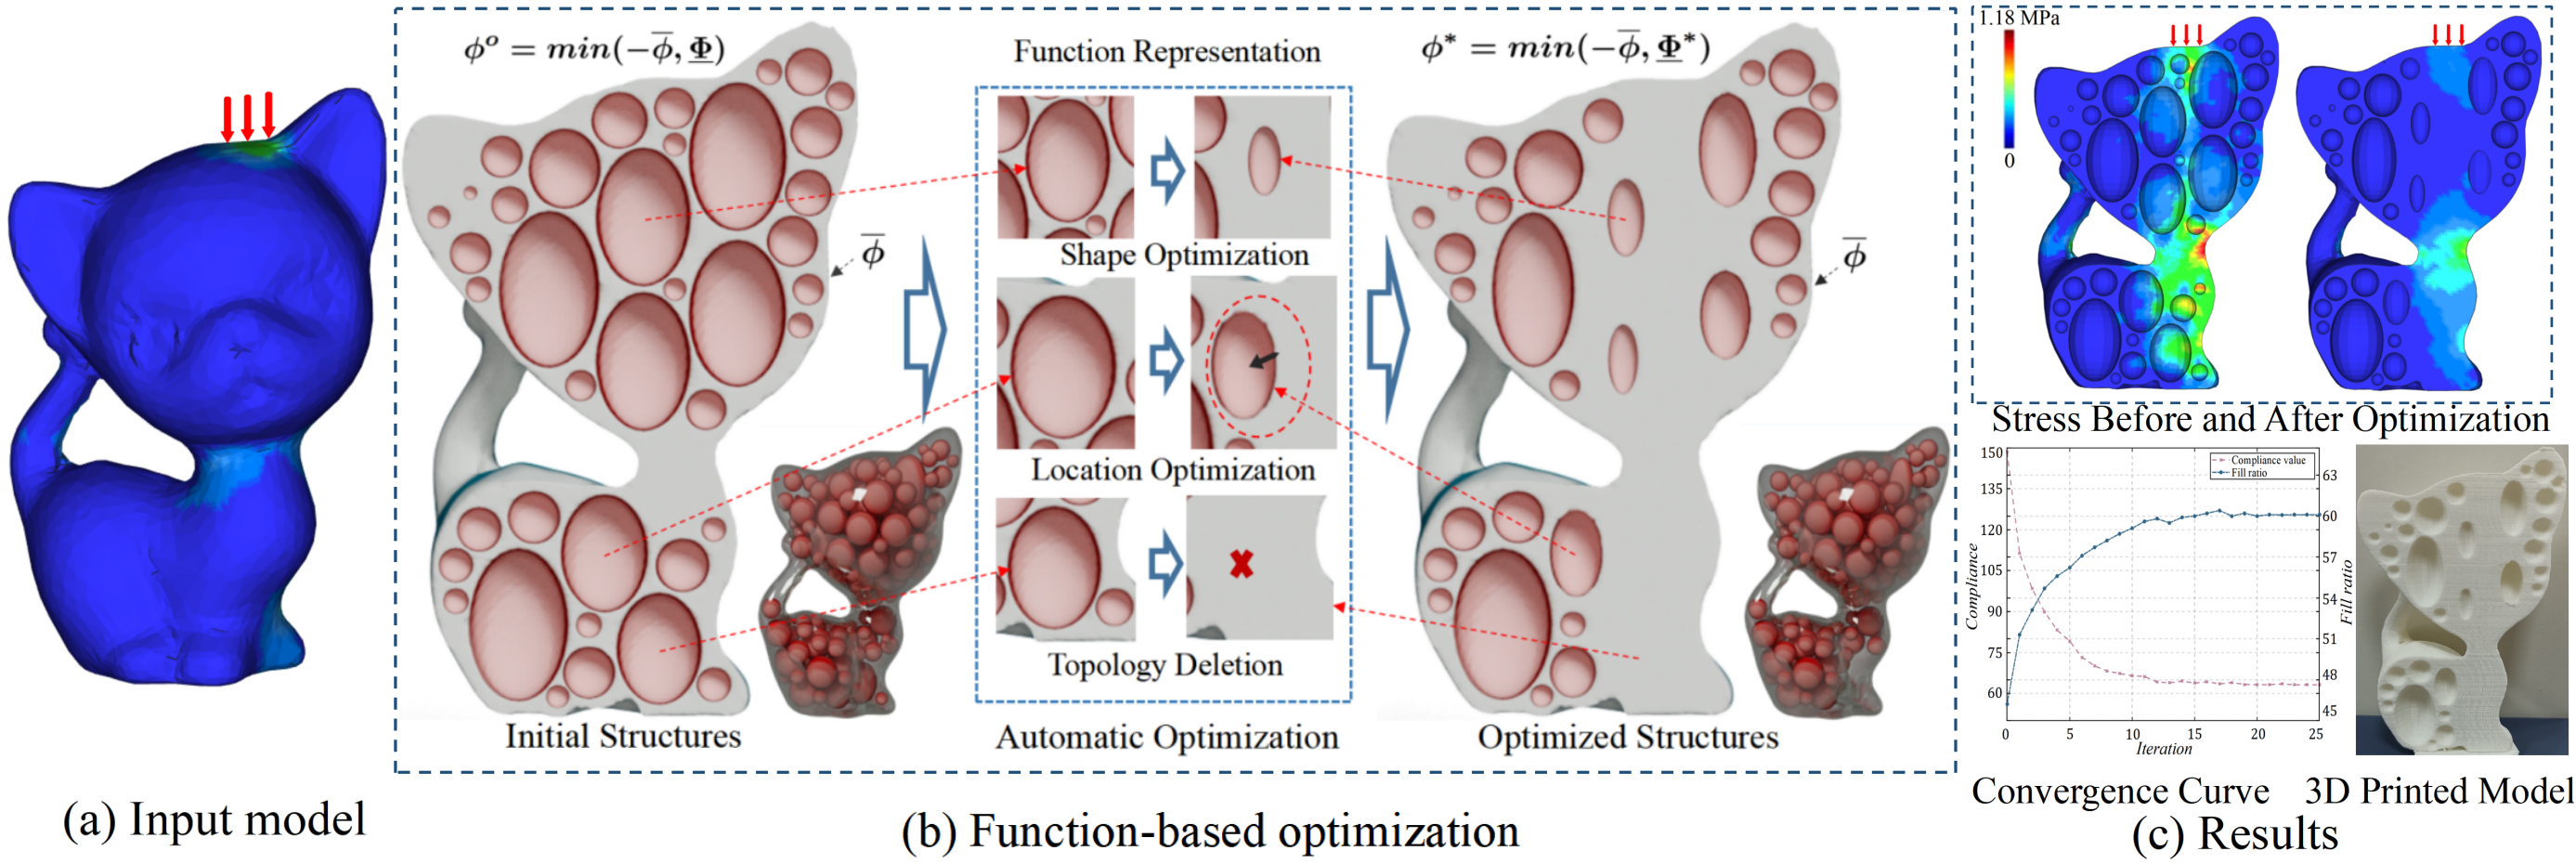
\includegraphics[width=0.95 \textwidth]{./figures/self-support/fig2.png}
  \caption{自支撑空心化算法流程图}
  \label{fig:1}
\end{figure*}

\section{研究方法}
以FDM 3D打印为例,在3D打印中有两个重要参数决定了打印模型的内部自支撑特性,分别是最大悬挑长度 $\delta_{0}$ 和最大悬挑角度 $\theta_{0}$,如图~\ref{fig:2}所示。这些与材料相关的参数 $\theta_{0}$ 和 $\delta_{0}$ 可通过实验测量得到。对于PLA材料,默认参数设置为 $\delta_{0}$ = 10mm 和 $\theta_0$ = $60^{\circ}$。

\subsection{自支撑空心结构设计}
本章算法在设计自支撑空心结构上,采用椭球体作为自支撑空腔结构,主要有两个原因:一是椭球体具有少量参数的显式函数表达式;二是可通过调整参数轻易实现自支撑。实际上,椭球体尺寸大小会影响其自支撑特性,如图~\ref{fig:2}所示。这意味着尺寸较小时,球体可无需支撑即可打印(图~\ref{fig:2} (b))。为更好描述自支撑椭球体问题,需引入一些定量参数:椭球体$E$在$X$、$Y$和$Z$轴上的三个主要半径分别为$a$、$b$和$c$;椭球体的打印方向默认与$z$轴对齐。为避免内部椭球体过小无法打印,设置$\min\{a, b\}> 5\sigma$,其中$\sigma$为每层制造厚度(默认$\sigma$=0.2 mm)。椭球体的下半球为自支撑,仅需考虑上半球。如图~\ref{fig:2} (a)所示,当悬挑角$\theta < \theta_{0}$时,相应部分为自支撑(低于红色水平线$p_1p_2$的部分)。对于悬挑角$\theta > \theta_{0}$的部分,若$p_1$和$p_2$间水平距离小于$\delta_{0}/2$,上方部分仍可自支撑。因此,可将椭球体自支撑的条件表述如下~\cite{lee2018support}:
\begin{equation}
  \begin{cases}
          a\leq c , \qquad &\text{if} \,\,  5\sigma \leq a \leq \delta_{0} / (2\ \cos\theta_{0}),                                       \\
          b\leq c , \qquad &\text{if} \,\,  5\sigma \leq b \leq \delta_{0} / (2\ \cos\theta_{0}),                                       \\
          c\geq a(4a^2-\delta^2_{0})^{\frac{1}{2}} \left. \middle/ \delta_{0}\ \tan\theta_{0} \right. \ \quad &\text{if} \, \, \, a > \delta_{0} / (2\ cos\theta_{0}),   \\
          c\geq b(4b^2-\delta^2_{0})^{\frac{1}{2}} \left. \middle/ \delta_{0}\ \tan\theta_{0} \right. \ \quad &\text{if} \, \, \, b > \delta_{0} / (2\ cos\theta_{0}). 
          \label{eq:1}
  \end{cases}
\end{equation}
\begin{figure}[htbp]
  \centering
  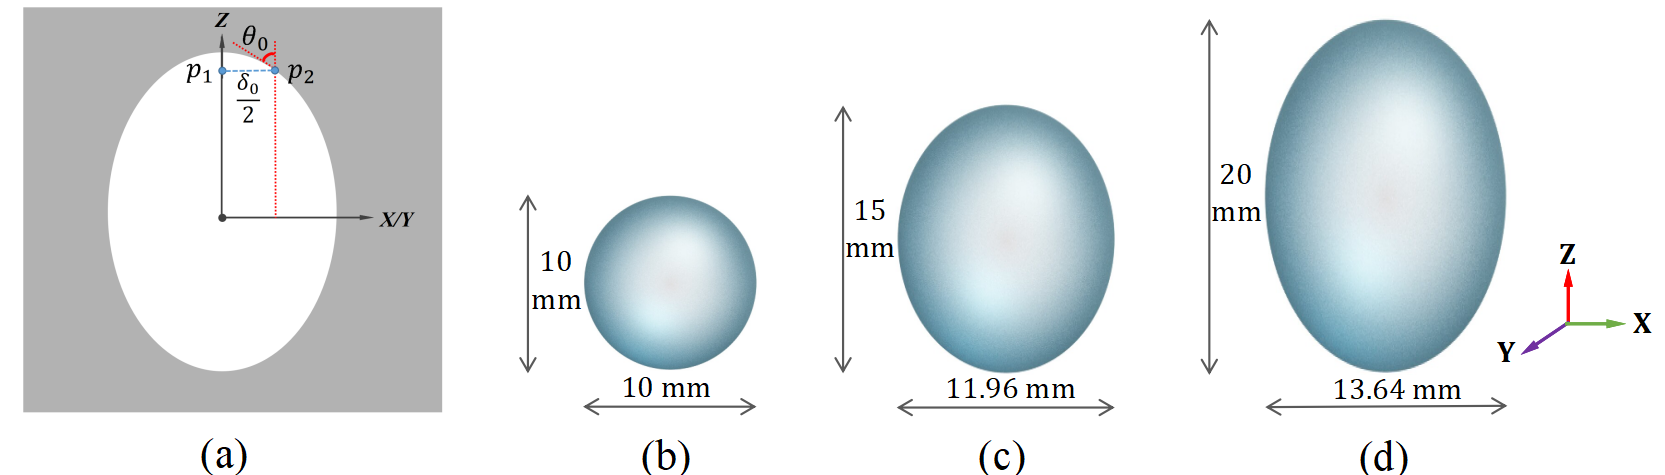
\includegraphics[trim={0 40 0 0},clip,width=0.65\textwidth]{./figures/self-support/fig3.png}\\
  \caption{自支撑椭球体示意图}
  \label{fig:2}
\end{figure}
对于固定主半径$c$的椭球体,可根据公式~(\ref{eq:1})调整另外两个半径$a$和$b$以获得自支撑的椭球体。图~\ref{fig:2} 还展示了具有不同尺寸的自支撑椭球体。在该方法中,确定可优化变量的范围对优化器很重要。

\subsection{自支撑空性化模型的函数表示}
相比离散边界表示,连续函数表示具有多方面优势,包括参数可控性、高精度、解析优化,以及易存储和传输。由于椭球体具有函数表示,可使用函数表示来描述具有椭球体空腔的模型。对于具有椭球体空腔的3D模型,可将其划分为模型的外表面和椭球体空腔的内部表面两部分,模型的外表面和内部表面均可使用函数进行隐式表示。
\begin{figure}[htbp]
  \begin {center}
  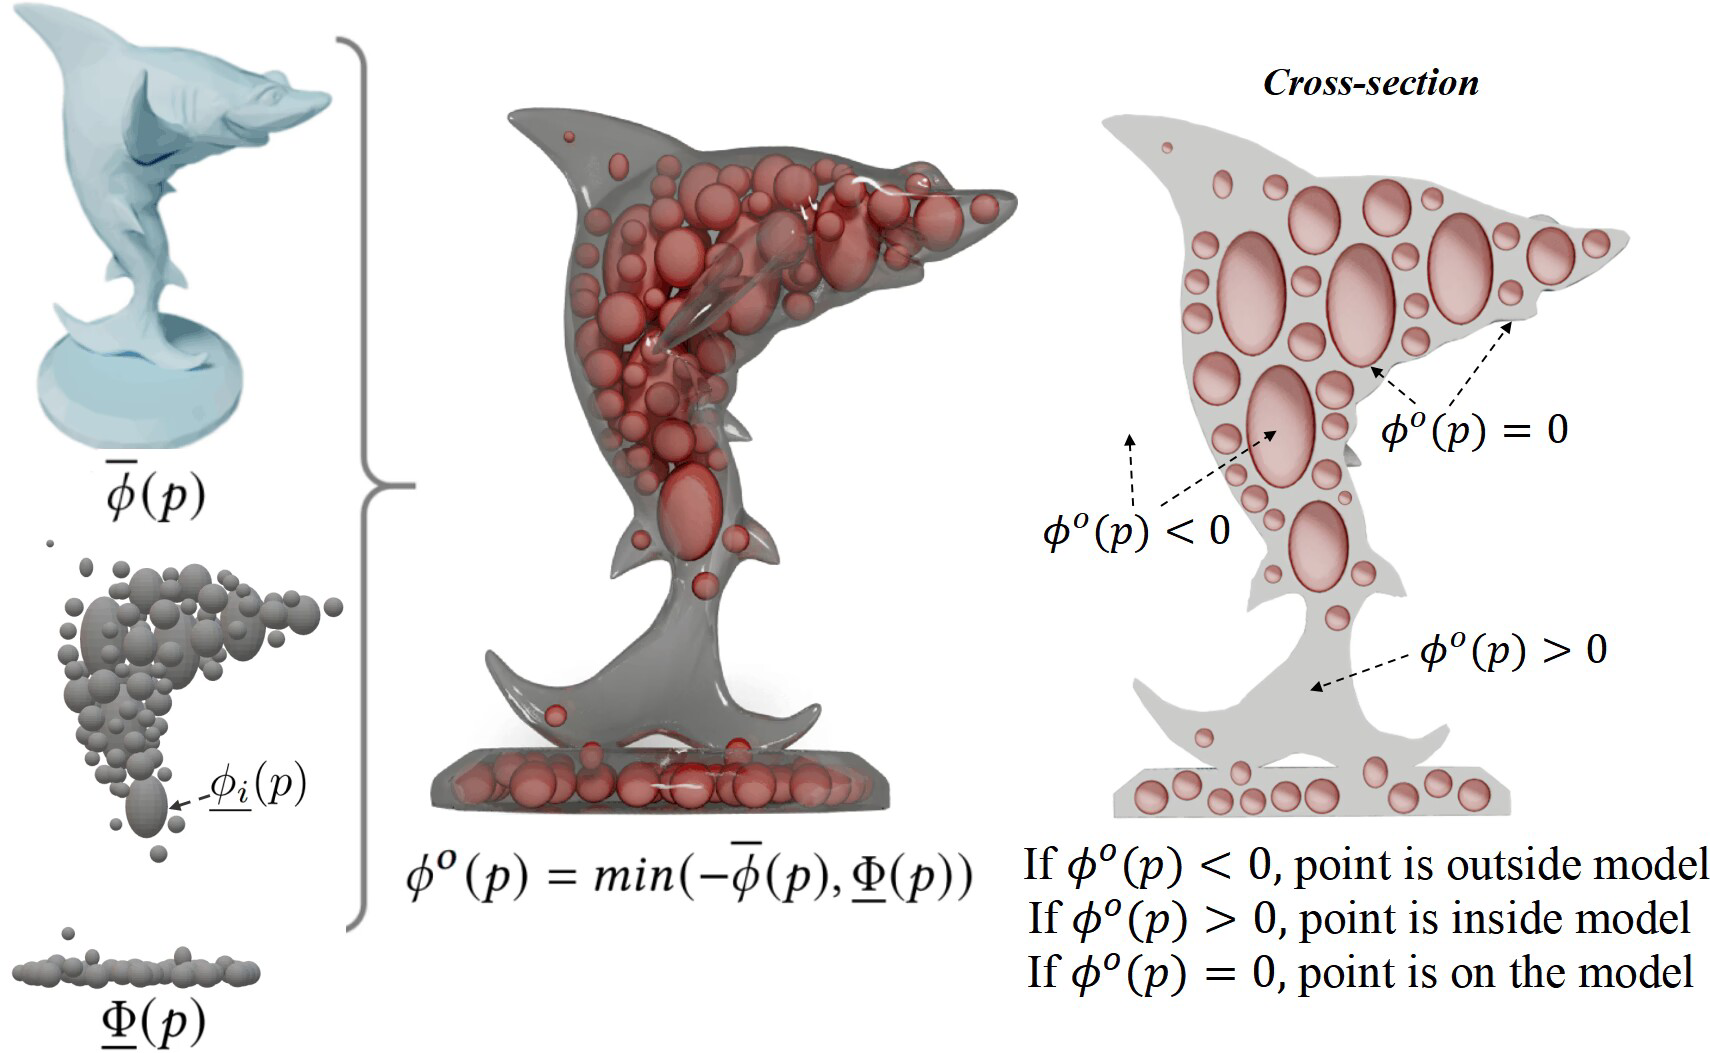
\includegraphics[width=0.65\textwidth]{./figures/self-support/fig4.png}
  \caption{椭球空心化3D模型的函数表示}
  \label{fig:3}
  \end {center}
\end{figure}

外表面可以用下面的径向基函数插值得到,
\begin{equation}
  \overline{\phi}(p)=\sum _{i=1}^{n_{t}}\alpha_{i}R_{i}(p)+Q(p),
  \label{eq:2}
\end{equation}
其中,$\overline{\phi}(p)$是模型的外表面函数,
$p=(x,y,z)$是设计空间中的一个点,
$R_{i}(p)=R(|p-p_{i}|)$是径向基核函数($R(x)=x^2log(|x|)$),
$\{p_{i}\}^{n_{t}}_{i=1}$是在模型表面上均匀采样的控制点集,
$n_{t}$是控制点的数量,
$Q(p)=\beta_{1}x+\beta_{2}y+\beta_{3}z+\beta_{4}$是一个单项式表达式,$\{\alpha_{i}\}$ 和 $\{\beta_{i}\} $ 是权重系数。
由于外表面无需改变,因此仅需对采样点和权重进行一次计算。该文采用RBF方法来逼近外表面,这是因为RBF具有强大的非线性拟合能力和高计算效率。当然,也可以考虑其他替代方案来实现相同的目标。

内表面通过椭球函数来表示,
\begin{equation}
  \begin{split}
      &\underline{\Phi}(p)=\min(\underline{\phi_{1}}(p), \underline{\phi_{2}}(p), \cdots, \underline{\phi_{n_e}}(p)),\qquad \quad
      \\
      &\underline{\phi_{i}}(p)=\frac{(x-x_{i})^2}{{a_i}^2}+\frac{(y-y_{i})^2}{{b_i}^2}+\frac{(z-z_{i})^2}{{c_i}^2}-1,
  \end{split}
  \label{eq:3}
\end{equation}
其中,$\underline{\Phi}(p)$表示椭球体空腔的整个内部表面,
$\underline{\phi_{i}}(p)$是第$i$个椭球体的表面,其三个主半径为($a_i$,$b_i$,$c_i$),中心点为$(x_{i},y_{i},z_{i})$,
${n_e}$是椭球体的数量,
$(x,y,z)$是椭球体的坐标,主半径和中心点用于控制椭球体,并根据目标需求进行优化。
然后,通过布尔运算可以获得具有椭球体空腔的3D模型的函数表示。具有椭球体空腔的3D模型的函数可表示为
\begin{equation}
  \phi^o(p)=\min(-\overline{\phi}(p), \underline{\Phi}(p) ). 
\end{equation}
函数表示可准确描述具有椭球体空腔的3D模型,并通过参数(如主半径和椭球体中心)控制其形状、位置和拓扑结构,图~\ref{fig:3}展示了具有椭球体空腔的模型表示。获得表示函数后,即可通过计算函数值轻松确定模型的内部和外部。若$\phi^o(p) < 0$,则点在模型外部;若$\phi^o(p) > 0$,则点在实体部分内部;若$\phi^o(p) = 0$,则点在模型表面上。连续可微函数有助于准确计算体积和进行高效敏感性分析,为自动优化提供可行条件。

\begin{figure}[t]
  \centering
  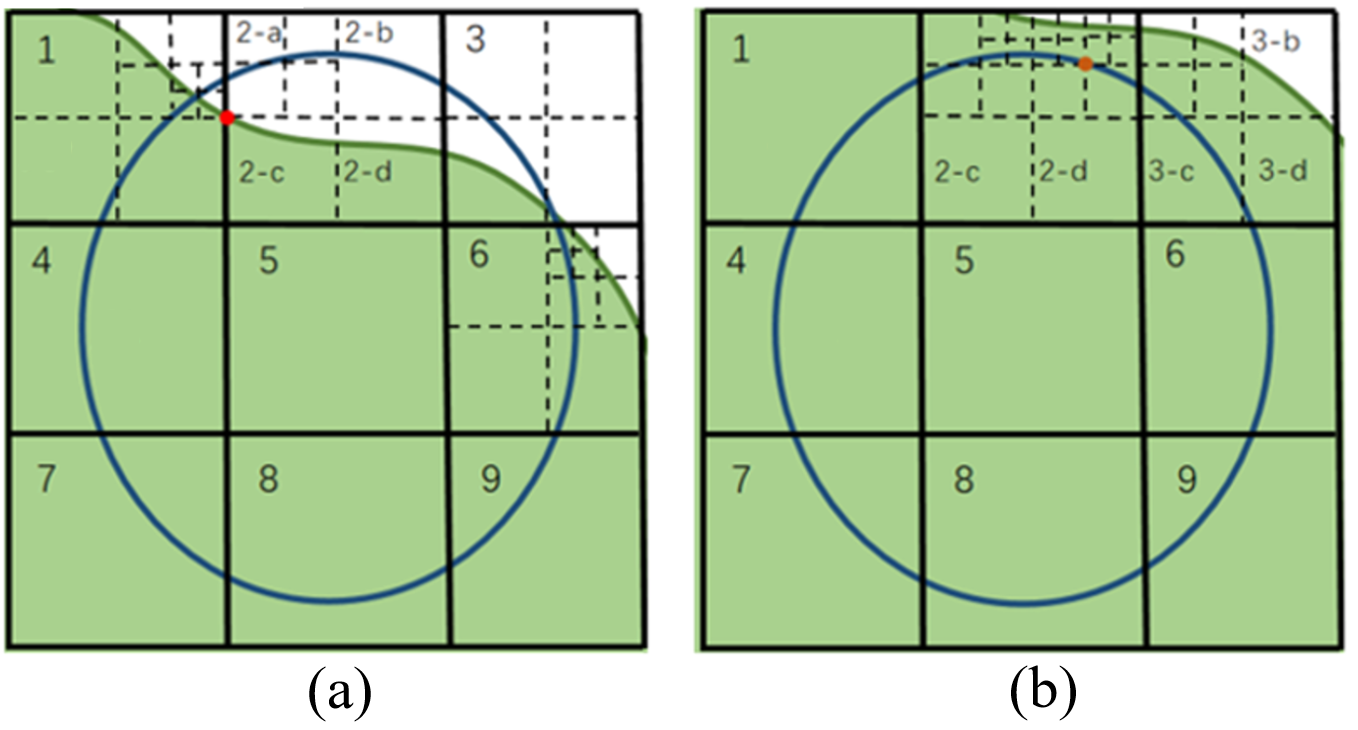
\includegraphics[width=0.6\textwidth]{./figures/self-support/fig6.png}
  \caption{2D视角下的自动定位示意图}
  \label{fig:5}
\end{figure}
\subsection{优化问题的形式及求解}
给定一个模型、外部载荷和体积约束,算法的目标是获得一个由椭球体组成的优化自支撑空腔的模型。所提出提出的问题形式和优化可以直接在函数上执行,无需耗时的重新网格化。结构柔度被用于制定优化目标,优化应变能以最大化结构刚度。在给定约束条件下,最小化具有自支撑空腔的模型顺应性可以表述如下:
\begin{equation}
  \begin{split}
      \min \quad  &I = \int_{\Omega_{D}} G(\phi^o(p))f \cdot u \, dV + \int_{\tau_{s}}F_{s} \cdot u\, dS ,     \\
      s.t.\quad  &\int_{\Omega_{M}} G(\phi^o(p)) \mathbb{E}:\, \varepsilon(u):\, \varepsilon(v)\, dV_{M}\\
      &= \int_{\Omega_{M}} G(\phi^o(p))f \cdot v \, dV  + \int_{\tau_{s}}F_{s} \cdot v\, dS,\,  \quad\forall v\in U_{ad},         \\
      & \int_{\Omega_{M}} G(\phi^o(p))\, dV< V_{c},                       \\
      & u = \overline{u} \quad on\quad \tau_{u},                       \\
      & d(\underline{\phi_{i}}(p), \underline{\phi_{j}}(p))>0,\forall \underline{\phi_{i}},\underline{\phi_{j}}\in\underline{\Phi},  \label{eq:7}
  \end{split}
\end{equation}
其中,$I$是结构顺应性,$\Omega_{D}$是设计域,$\Omega_{M}$是模型域,$G(*)$是正则化的Heaviside函数\cite{hu2020efficient},$f$是体积力,$F_{s}$是定义在Neumann边界$\tau_{s}$上的表面拉力,$v$是定义在$\Omega_{D}$上的相应测试函数,其中$U_{ad} = {v|v\in Sob_{1}(\Omega_{M}), v = 0 , on ,\tau_{u}}$,$u$是位移场,$Sob_{1}$是一阶Sobolev空间,$\varepsilon$是二阶线性应变张量,$\mathbb{E}$是由弹性模量和泊松比决定的四阶各向同性弹性恒等张量,$\overline{u}$是在Dirichlet边界$\tau_{u}$上的预设位移,$V_{c}$是体积约束,$d(\phi_{i}(p), \phi_{j}(p))$是第$i$个椭球体和第$j$个椭球体之间的距离。
\begin{figure}[t]
  \centering
  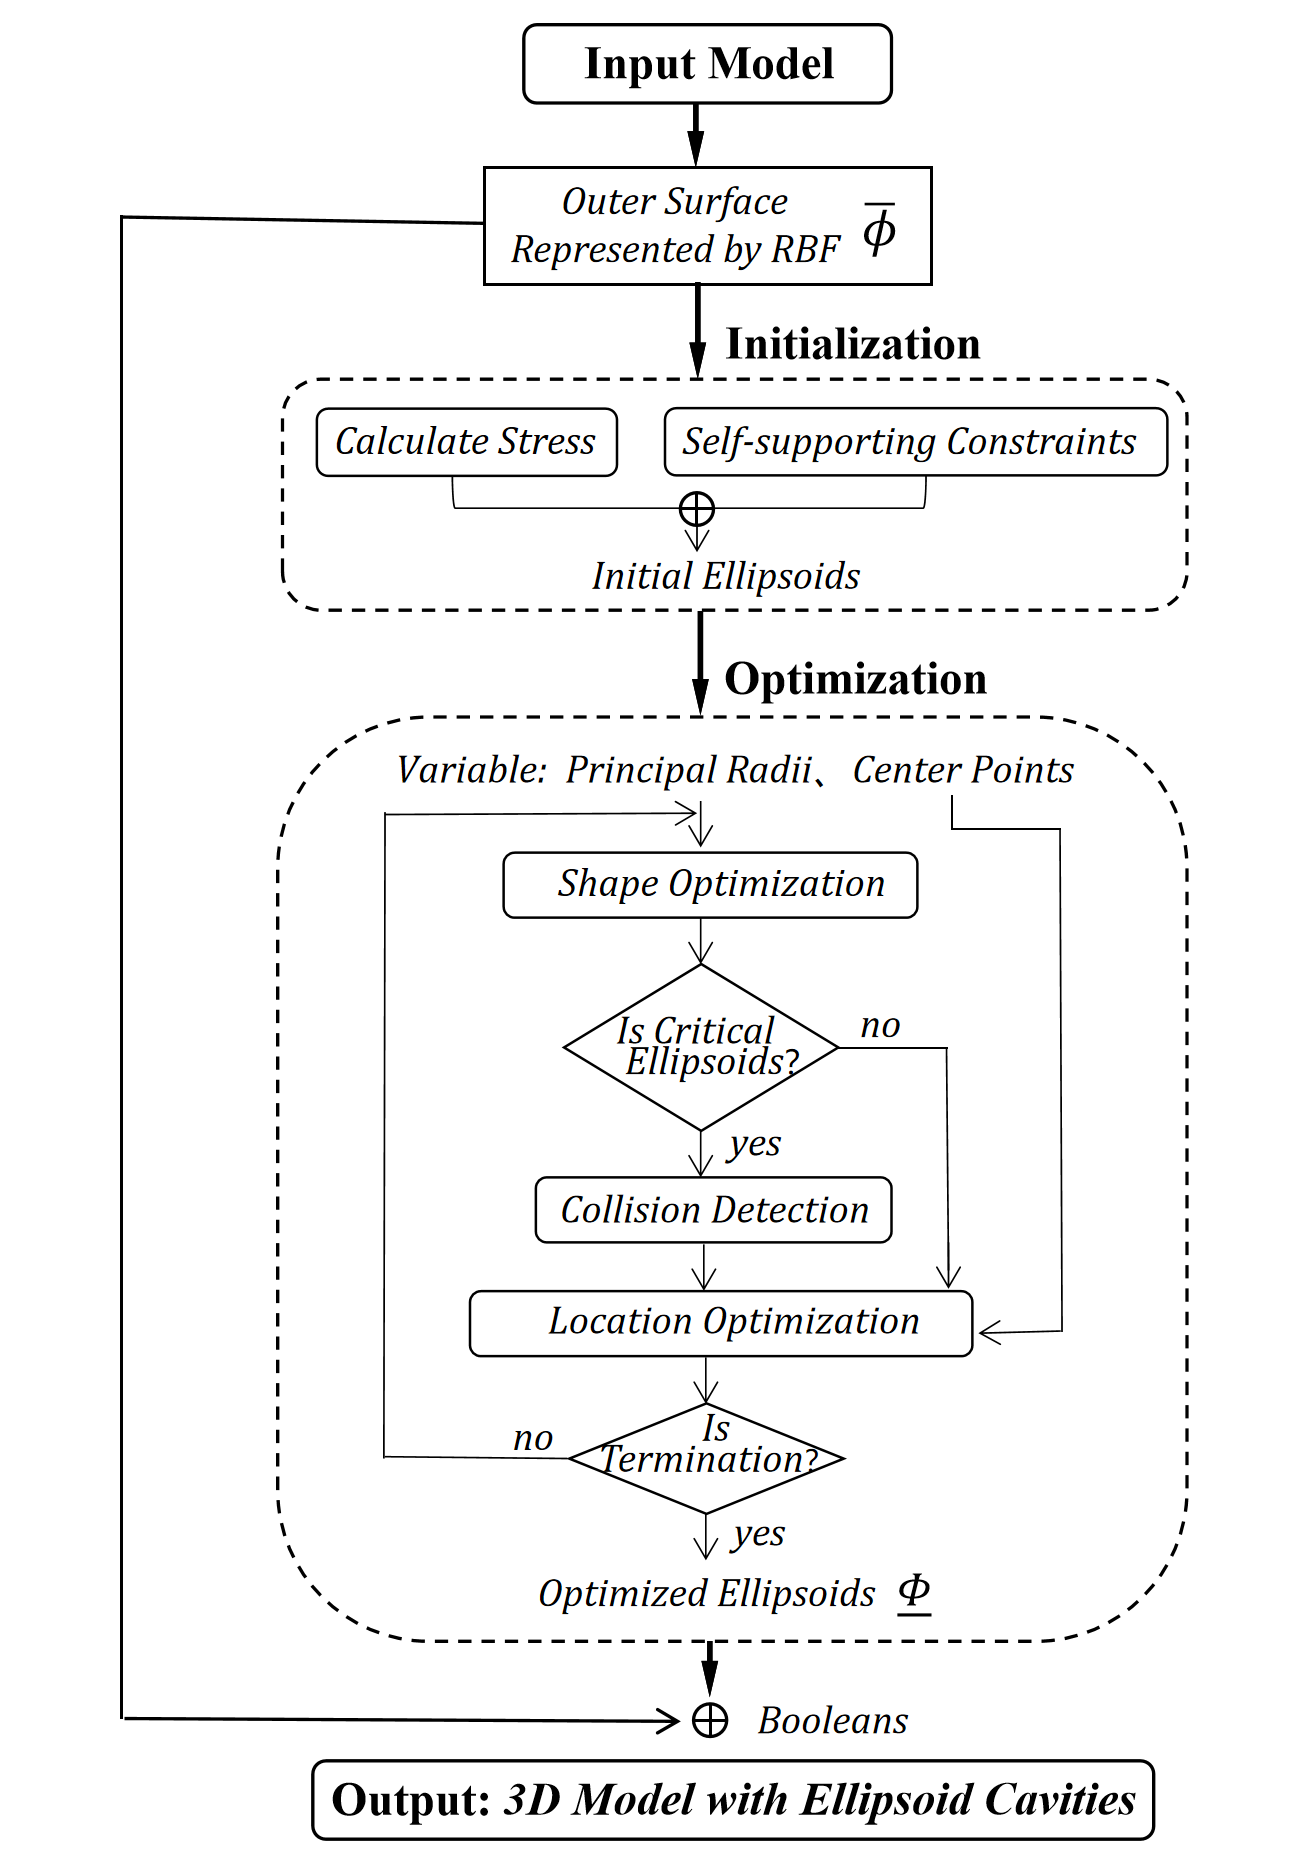
\includegraphics[height=4in]{./figures/self-support/fig17.png}
  \caption{算法流程}
  \label{fig:algo}
\end{figure}

\begin{figure*}[htbp]
  \centering
  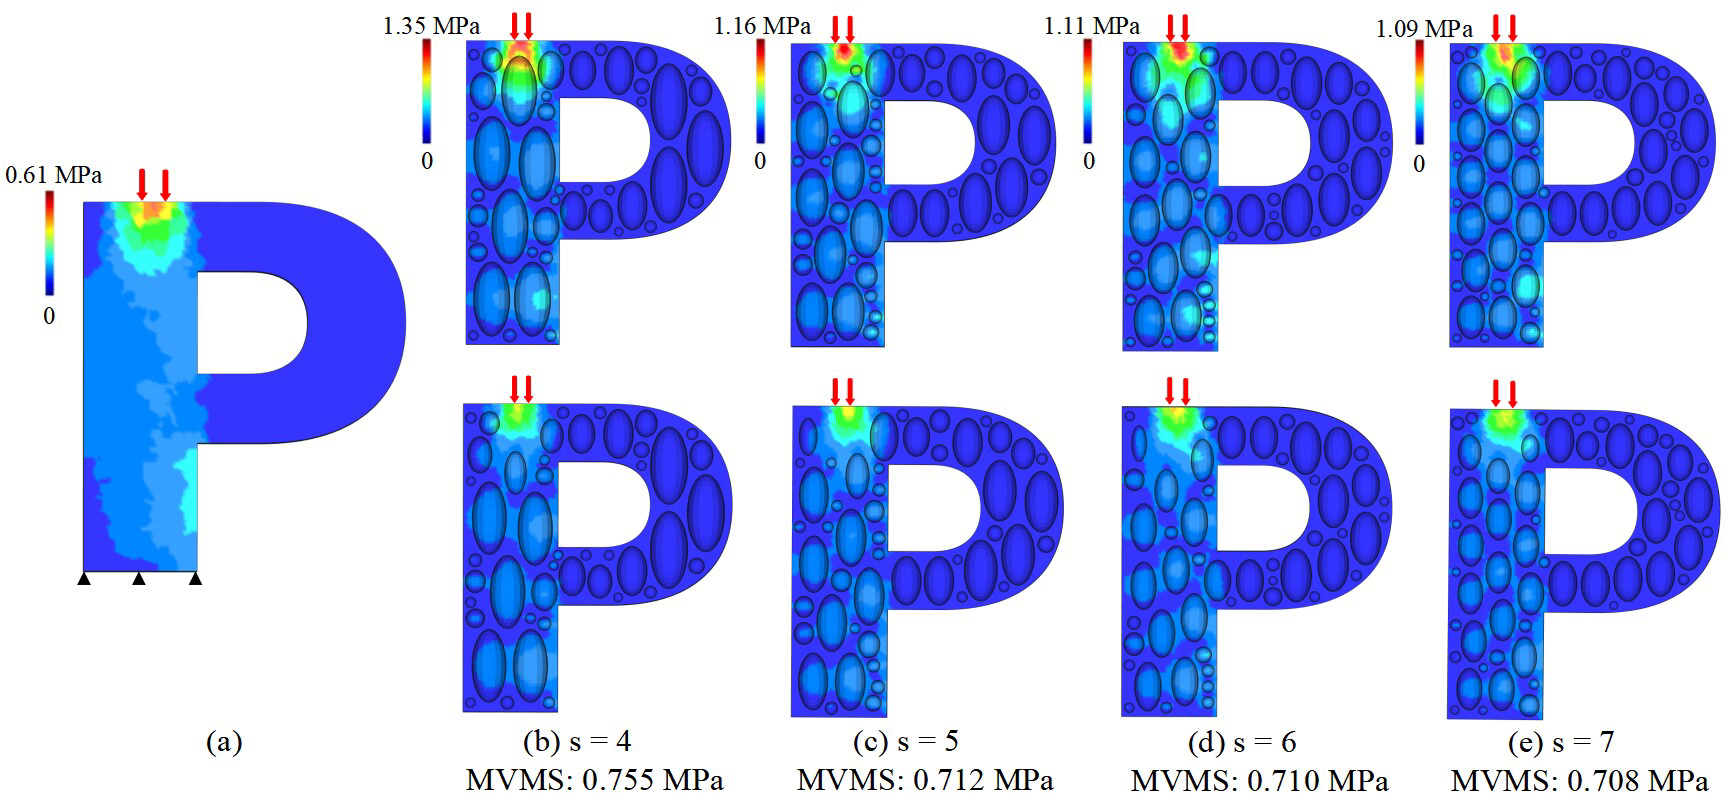
\includegraphics[width=1.0 \textwidth]{./figures/self-support/fig7.png}
  \caption{尺寸参数 $s$ 的影响}
  \label{fig:6}
\end{figure*}
优化的主要目标是在满足目标体积约束的前提下,提高结构的物理性能,而非仅关注实现自支撑特性。结构的自支撑特性在初始化阶段即已确立,在优化过程中,通过限制主半径最大范围来确保自支撑能力,该方法有助于减少优化过程中的约束条件数量。

\paragraph{问题的离散化。}
与传统有限元分析不同,每次迭代都需要对四面体或六面体网格进行重网格化来描述形状并计算,而重网格化过程非常耗时,且容易出现网格失败或质量较差的问题。在本章方法中,形状由连续函数描述,仅需构建一次统一的有限六面体单元作为积分域,并在整个优化过程中保持六面体单元不变。方程~\ref{eq:7}中的优化问题可重写为离散形式,
\begin{equation}
\centering
    \begin{split}
        \min \quad & I = U^{T} K U,   \\
        s.t. \quad & K U = F,       \\
        &V = \frac{1}{8}\sum _{i=1}^{n} \sum _{j=1}^{8}G(\overline{\phi}_{i,j})- \sum _{k=1}^{n_{e}} \frac{4}{3} \pi a_{k} b_{k} c_{k} \leq V_{c}, \\
        &\sum _{i=1}^{n_{e}} \sum _{j=1}^{n_{e}-1}E_{s}^{ij}=0, 
    \end{split}
    \label{eq:9}
\end{equation}
其中$U$是位移矩阵,$F$是体力向量,$n$是用于积分计算的离散单元数量,$n_{e}$是椭球体空腔的数量,$V_{c}$是体积约束,$\overline{\phi}{i,j}$是第$i$个单元的第$j$个节点点处$\overline{\phi}(*)$的值,$K$是刚度矩阵,其中$K_i$是第$i$个单元的刚度矩阵,($a_k$,$b_k$,$c_k$)是第$k$个椭球体的三个主半径,$E{s}^{ij}$是第$i$个椭球体与第$j$个椭球体之间的碰撞检测。

\subsection{优化求解过程}
良好的初始化有助于加快优化收敛,本节提供了一种基于输入模型结构强度构建的应力初始化方法。给定均匀采样的椭球体质心,目标是获得一个无交叉的自支撑椭球体填充。根据公式 (\ref{eq:1}) 中的自支撑计算,仅需获得每个椭球体的主半径$c$,其他两个主半径$a$和$b$的最大值可以推导得出。第$i$个椭球体的主半径$c_i$可计算为
\begin{equation}
  c_{i} = e^{-{(2\sigma_{n}})^2}*\frac{h_{max}}{s},
  \label{eq:6}
\end{equation}
其中,$\sigma_n$为标准化结构应力,$h_{max}$为输入模型最大高度,$s$为调整自支撑椭球体大小和数量的缩放因子。缩放因子$s$影响椭球体空腔大小和数量,但对优化结构力学性能影响较小。在相同填充比下,缩放因子$s$越大,椭球体空腔数量越多。当缩放因子$s$取6时,在结构强度和椭球体数量间达到了良好平衡,如图~\ref{fig:6}所示。获得椭球体初始主半径后,将使用自动定位检测调整椭球体大小。当无相交椭球体时,即可获得初始化。


$n_e$个椭球体的变量包括主半径${(a_i,b_i,c_i)}{i=1}^{n_e}$和中心点${(x_i,y_i,z_i)}{i=1}^{n_e}$。在优化过程中,如果未施加限制,椭球体很可能发生碰撞,这种碰撞会损害结构的自支撑性能。为解决这一问题,可采用GJK算法~\cite{gilbert1988fast}检测椭球体间碰撞,并计算每个椭球体的可行运动范围,确保无碰撞运动。

为避免优化迭代中椭球体频繁碰撞,设置了设计变量上限,将椭球体限制在各自可行范围内。然而,在每次迭代中重新计算每个椭球体可行范围会带来大量额外计算开销。实际上,无需在单次迭代中求解所有椭球体可行范围。大多数椭球体在优化过程中保持不变,无需进行碰撞检测。通过排除这些不变椭球体,可提高计算效率,并保持优化问题可微分性。剩余的被称为关键椭球体的,是根据上次迭代梯度值确定的。在迭代过程中,仅监测涉及关键椭球体的碰撞。初始时通常仅有少数关键椭球体,在优化过程中数量逐渐增加,但相对保持较小。

每步迭代, 形状参数 $\{(a_i,b_i,c_i)\}^{n_e}_{i=1}$ 首先被优化,局部参数 $\{(x_i,y_i,z_i)\}^{n_e}_{i=1}$ 先固定。目标函数关于变量的梯度可以计算得到:
\begin{equation}
  \begin{split}
      &\frac{\partial I}{\partial t_{k}} =-U^T\frac{\partial K}{\partial t_{k}}U=-U^T[{\frac{1}{8}}\sum_{i=1}^{n} \sum_{j=1}^{8}q(G(\phi^{o}_{ij}))^{q-1}\frac{\partial {G(\phi^{o}_{ij})}}{\partial t_{k}}K_{i}]U,               \\
      &\frac{\partial V}{\partial t_{k}} = \sum_{k=1}^{n_{e}} \frac{4}{3} \pi \frac{a_{k}b_{k}c_{k}}{t_{k}},  \ \\
      &\frac{\partial G(\phi^{o}_{ij})}{\partial t_{k}} = \frac{\partial G}{\partial \phi^{o}_{ij}} \dot \frac{\partial \phi^{o}_{ij}}{\partial t_{k}}, 
  \end{split}
\end{equation}
其中,$t_k$表示待优化参数,可以采用移动渐近线优化器~\cite{svanberg1987method}中的相应$\partial I / \partial t_{k}$来更新形状参数${(a_i,b_i,c_i)}_{i=1}^{n_e}$。如果某个椭球体更新后的形状参数最小值低于第3.1节提到的指定阈值,则将其移除,并将椭球体数量更新为$n_e=n_e-1$。
接下来,采用类似的方法优化位置参数${(x_i,y_i,z_i)}_{i=1}^{n_e}$,同时保持更新后的形状参数固定不变。
尽管无法通过数学推导保证收敛,但在实验中,所有结果都在数十次迭代内收敛。

\begin{figure*}[htbp]
  \begin {center}
  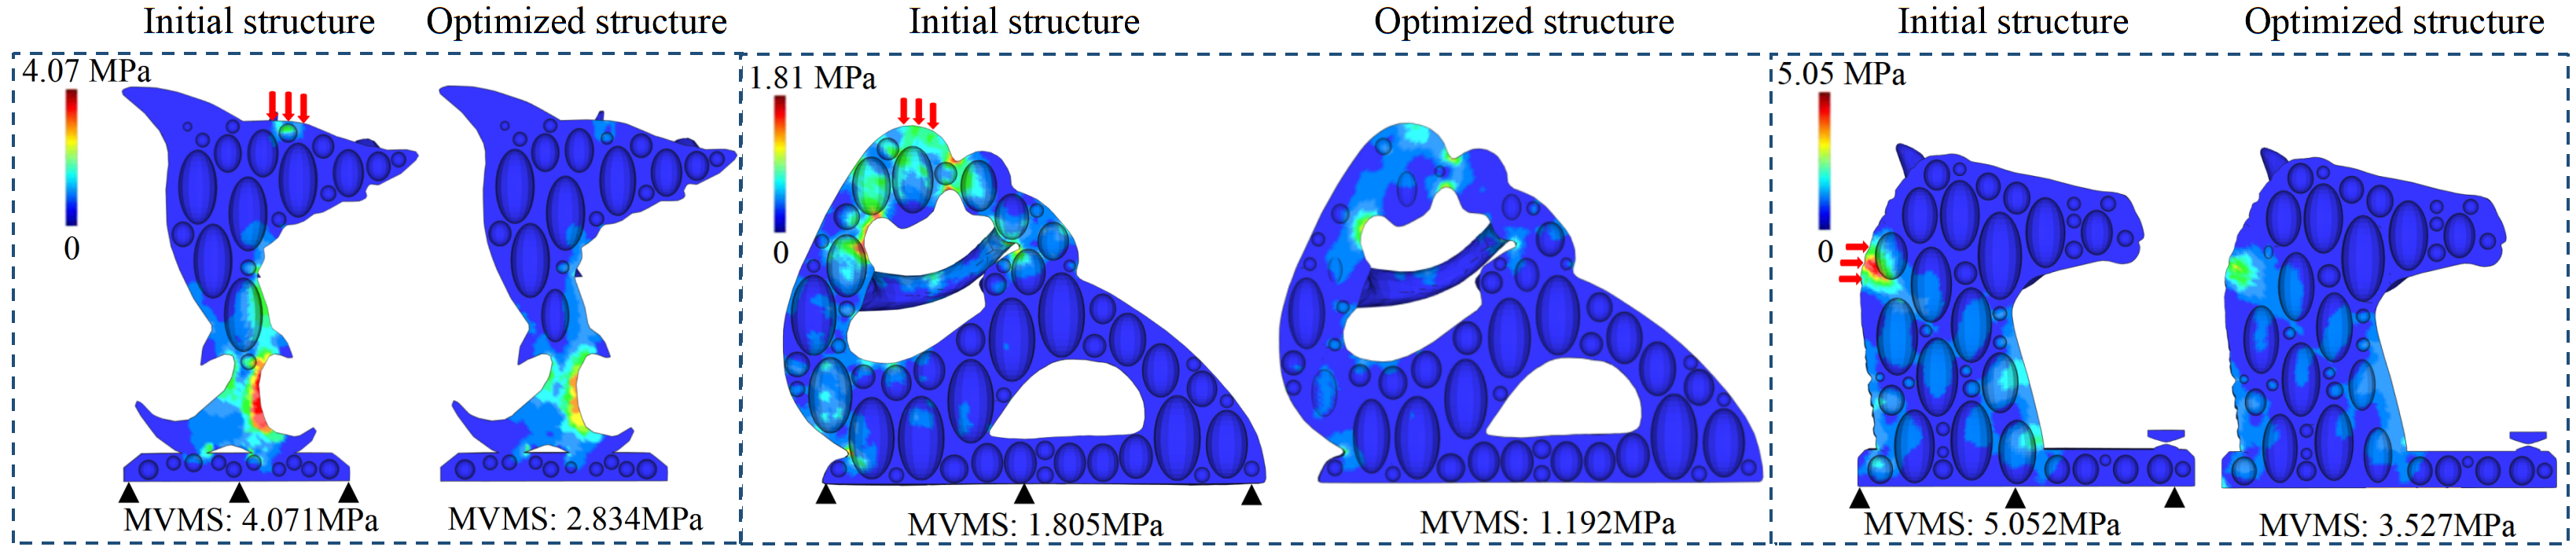
\includegraphics[width=0.98 \textwidth]{./figures/self-support/fig8.png}
  \caption{初始结构和优化结构的应力分布比较}
  \label{fig:7}
  \end {center}
\end{figure*}

\begin{figure}[htbp]
  \begin {center}
  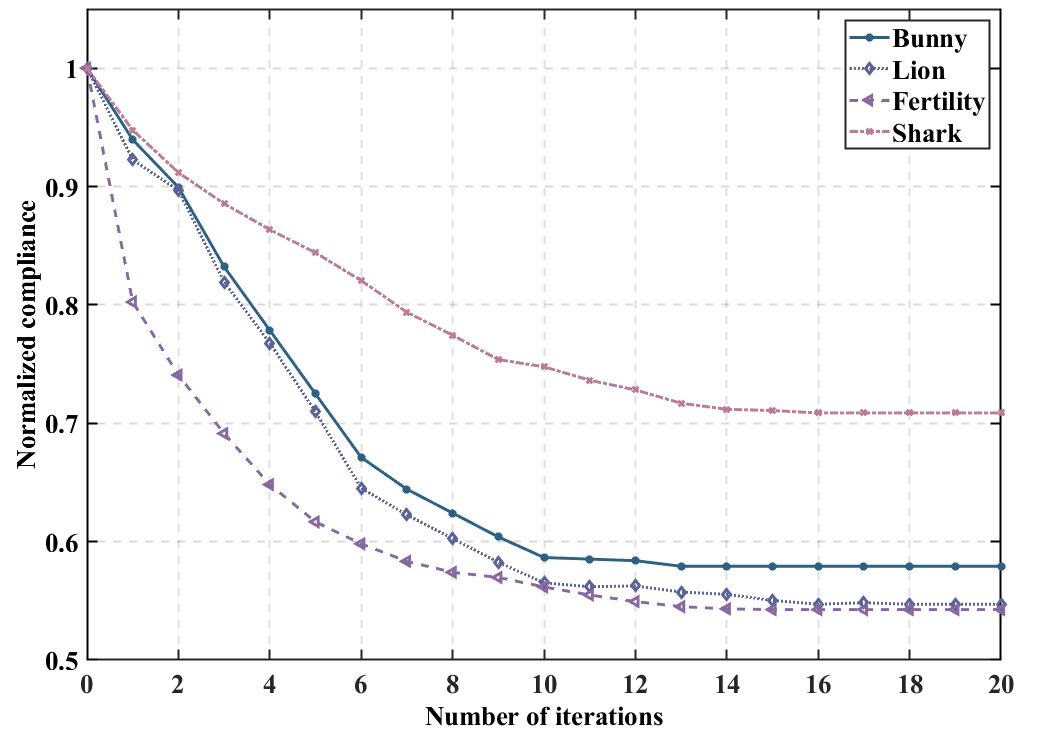
\includegraphics[width=0.6 \linewidth]{./figures/self-support/fig9.png}
  \caption{四个模型的收敛曲线}
  \label{fig:8}
  \end {center}
\end{figure}

\section{实验和讨论}
本节测试了所提出的自支撑空心化方法在各个方面的性能。默认情况下,在固定底部的情况下,在顶部施加1.0 $N/mm^2$的表面压力。填充的自支撑结构由3D打印机使用0.2 mm的切片厚度和弹性模量为3000 MPa、泊松比为0.35的PLA塑料打印。
设计和优化过程中涉及一些参数,其中大部分参数与模型无关,可以默认固定。所有实验均在一台配备3.70GHz Intel(R)Core(TM) i9-10900 CPU和128 GB RAM的计算机上进行。

\begin{figure}[htbp]
  \begin {center}
  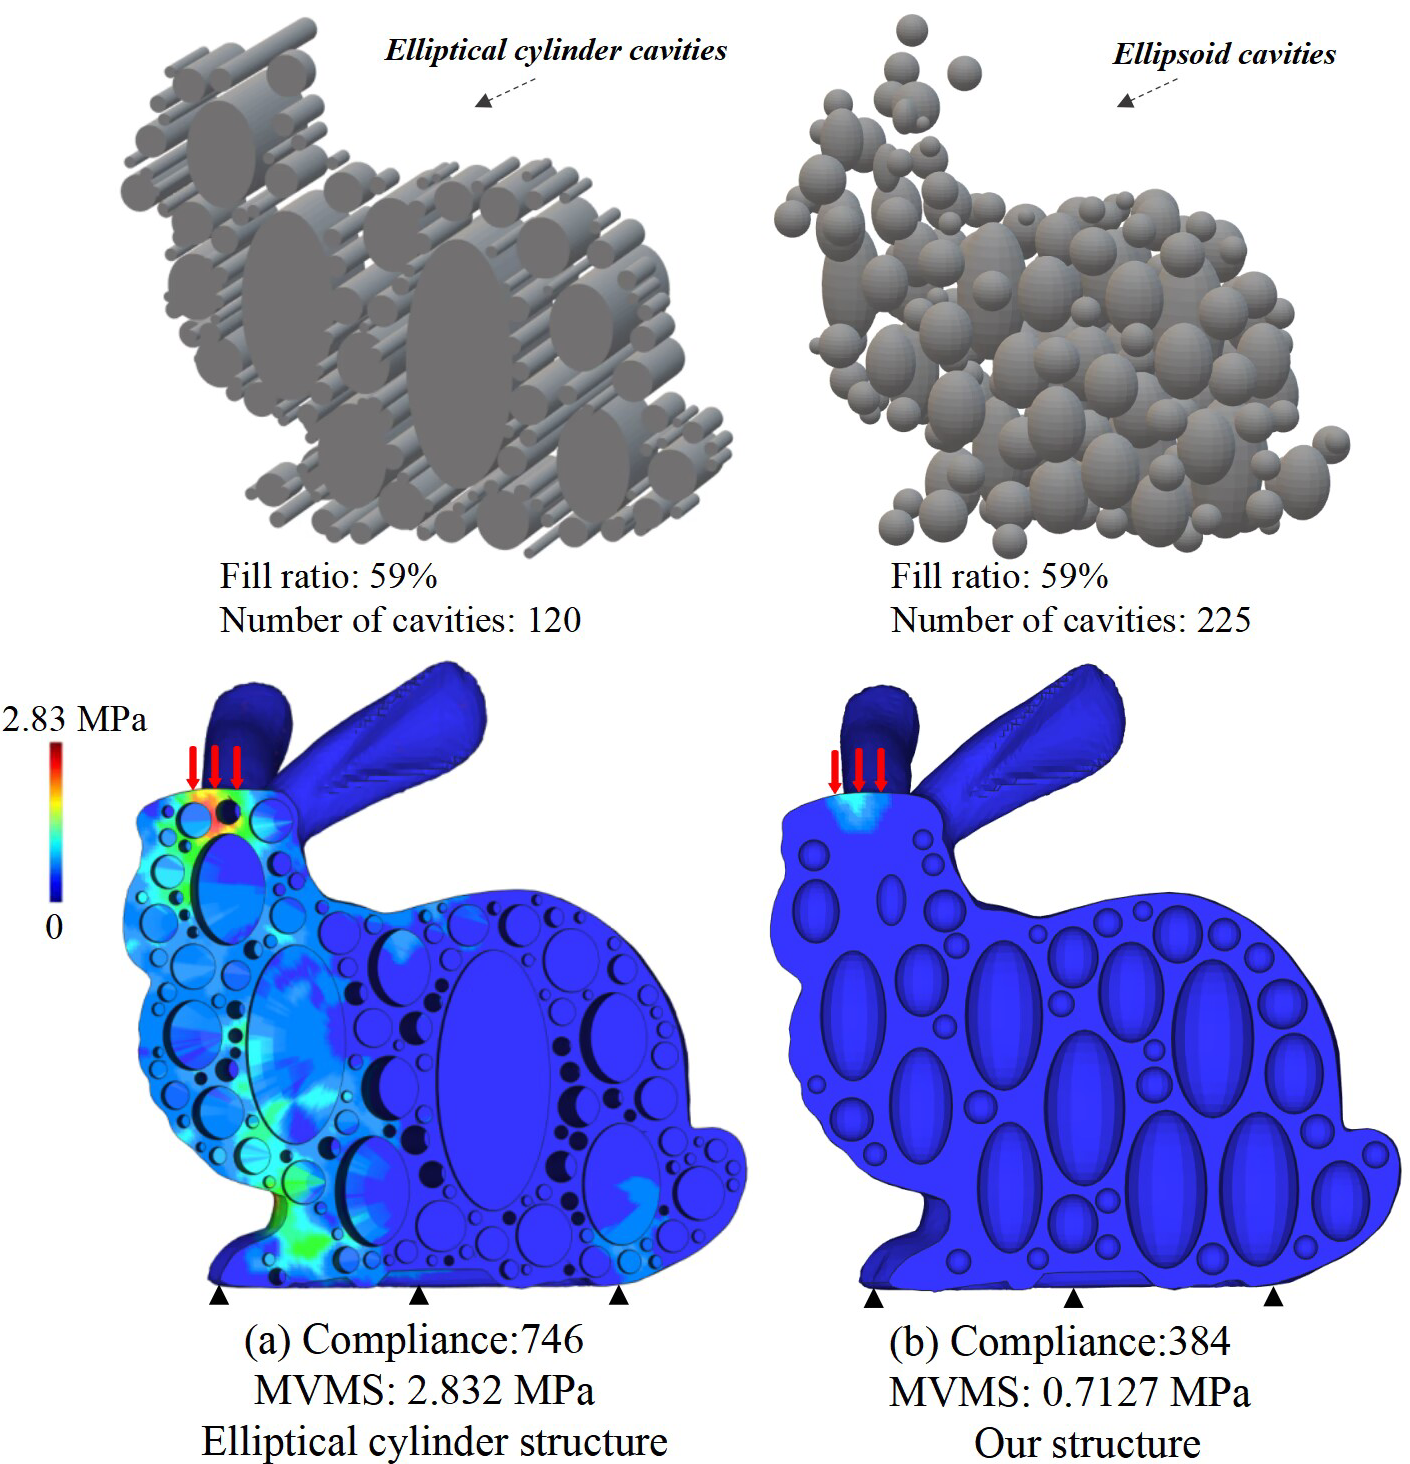
\includegraphics[width=0.65 \textwidth]{./figures/self-support/fig10.png}
  \caption{与椭圆柱体结构方法 \cite{lee2018support} 在相同填充比例下的比较实验 }
  \label{fig:9}
  \end {center}
\end{figure}

\subsection{有效性和效率性}
众所周知,在基于传统有限元分析(FEA)的优化方法中,生成四面体网格和/或六面体网格需要耗费大量时间。而且在传统基于FEM的优化过程中,重新网格化是必需的步骤,用于表示形状并执行计算。
相比之下,基于函数的3D模型表示方法可以直接在离散计算中对这些函数进行积分和梯度计算,仅需构建一次简单的均匀有限元作为积分域即可。在建模和优化过程中不需要频繁重新网格化,这导致数值计算非常高效和稳定,特别是对于大型复杂结构。
图~\ref{fig:7}显示了初始化和相应的优化结果。所提出的方法生成了轻量级且强度高的模型,这些模型通过优化的自支撑椭球体进行了空心化,并具有良好的力学性能。相应模型的时间和优化数据如表~\ref{T:table1}所示。在几何(形状和位置)和拓扑(空腔数量)优化后,最大冯·米塞斯应力(MVMS)得到了显著改善。
使用传统有限元分析很难获得优化的椭球体,这里仅列出了FEA中一次迭代的计算时间。所提出的方法更加高效,所有实验都在数十步内收敛,总时间(包括初始化和优化)每个模型不到一小时。

此外,所提出的基于函数的框架提供了精确的解析梯度,并确保了优化的数值稳定性。图~\ref{fig:8}展示了四种不同模型的收敛曲线。为了直观显示,收敛曲线已经通过刚度能量进行了归一化处理,这些模型均在20次迭代内实现了收敛。


\begin{table*}
    \centering
    \fontsize{7.5}{8}\selectfont
    \caption{实验结果表:优化数据和时间 }
    \label{T:table1}
    % Please add the following required packages to your document preamble:
    % \usepackage{multirow}
    \renewcommand{\arraystretch}{1.5}
    \setlength{\tabcolsep}{1.2mm}{
    \resizebox{1.0\linewidth}{!}{
        \begin{tabular}{c|ccc|ccc|cc|c|clllll}
            \cline{1-11}
            \multirow{2}{*}{\textbf{模型}} & \multicolumn{3}{c|}{\textbf{初始空心化模型}} & \multicolumn{3}{c|}{\textbf{优化空心化模型}} & \multicolumn{2}{c|}{\textbf{优化}} & \multirow{2}{*}{\textbf{总时间}(min)} & \multirow{2}{*}{\textbf{一步FEA时间}(min)} & \multicolumn{2}{c}{} & \multicolumn{1}{c}{}          & \multicolumn{1}{c}{\multirow{2}{*}{}} & \multicolumn{1}{c}{\multirow{2}{*}{}}                                                                                   \\ \cline{2-9}
                                   & \multicolumn{1}{c}{MVMS(MPa)}             & \multicolumn{1}{c}{\# Ellipsoids}           & Fill ratio                        & \multicolumn{1}{c}{MVMS(MPa)}    & \multicolumn{1}{c}{\# Ellipsoids}  & Fill ratio           & \multicolumn{1}{c}{Time(min)} & \#iterations                          &                                       &      & \multicolumn{1}{c}{} &  &  & \multicolumn{1}{c}{} & \multicolumn{1}{c}{} \\ \cline{1-11}
            P                      & \multicolumn{1}{c}{1.11}                  & \multicolumn{1}{c}{228}                     & 55.6\%                            & \multicolumn{1}{c}{0.71}         & \multicolumn{1}{c}{219}            & 59.47\%              & \multicolumn{1}{c}{2.31}      & 20                                    & 52.6                                  & 4.22 &                      &  &  &                      &                      \\
            Bunny                  & \multicolumn{1}{c}{1.49}                  & \multicolumn{1}{c}{231}                     & 54.21\%                           & \multicolumn{1}{c}{0.713}        & \multicolumn{1}{c}{225}            & 59.03\%              & \multicolumn{1}{c}{2.26}      & 16                                    & 46.2                                  & 3.67 &                      &  &  &                      &                      \\
            Shark                  & \multicolumn{1}{c}{4.07}                  & \multicolumn{1}{c}{213}                     & 62.31\%                           & \multicolumn{1}{c}{2.83}         & \multicolumn{1}{c}{208}            & 65.02\%              & \multicolumn{1}{c}{2.24}      & 17                                    & 42.6                                  & 3.18 &                      &  &  &                      &                      \\
            Fertility              & \multicolumn{1}{c}{1.81}                  & \multicolumn{1}{c}{193}                     & 59.42\%                           & \multicolumn{1}{c}{1.19}         & \multicolumn{1}{c}{183}            & 64.98\%              & \multicolumn{1}{c}{2.21}      & 16                                    & 41.4                                  & 3.25 &                      &  &  &                      &                      \\
            Molar                  & \multicolumn{1}{c}{8.92}                  & \multicolumn{1}{c}{330}                     & 50.54\%                           & \multicolumn{1}{c}{5.94}         & \multicolumn{1}{c}{329}            & 55.81\%              & \multicolumn{1}{c}{2.37}      & 18                                    & 53.9                                  & 3.75 &                      &  &  &                      &                      \\
            Kitten                 & \multicolumn{1}{c}{2.58}                  & \multicolumn{1}{c}{413}                     & 42.27\%                           & \multicolumn{1}{c}{1.59}         & \multicolumn{1}{c}{402}            & 54.48\%              & \multicolumn{1}{c}{2.41}      & 18                                    & 52.2                                  & 4.03 &                      &  &  &                      &                      \\

            Horse                  & \multicolumn{1}{c}{5.05}                  & \multicolumn{1}{c}{567}                     & 38.42\%                           & \multicolumn{1}{c}{3.51}         & \multicolumn{1}{c}{564}            & 41.5\%               & \multicolumn{1}{c}{2.54}      & 16                                    & 46.7                                  & 3.53 &                      &  &  &                      &                      \\ \cline{1-11}
        \end{tabular}}}
\end{table*}


\subsection{比较和讨论}
为验证所提出方法的有效性,结果与最相关的椭圆柱结构~\cite{lee2018support}进行了比较。
椭圆柱方法使用贪心初始化生成空腔结构,但无法优化相应结构。此外,椭圆柱结构由2D椭圆拉伸而成,在具有复杂几何和拓扑的形状中会出现空心化问题。所提出的椭球体在3D空间中构建,具有更高的自由度,轴长和位置可以使用高效的无网格方法进行优化。优化后的结构明显优于~\cite{lee2018support}方法的结果。
柔度反映了整体结构强度,最大冯·米塞斯应力(MVMS)用于反映结构中最薄弱的局部区域。结构柔度或MVMS越小,结构越强。
如图~\ref{fig:9}所示,椭圆柱结构和所提出结构的顺应性分别为746和384,两种结构的MVMS分别为2.832 MPa和0.7127 MPa。这表明,在相同条件(外载和体积约束)下,所提出结构的刚度明显优于椭圆柱结构。

本文还与与其他相关方法进行了比较,包括菱形结构~\cite{wu2016self}、三角-六边形结构~\cite{xu2021support}、基于TPMS的结构~\cite{hu2020efficient}和蜂窝结构~\cite{10.1145/2601097.2601168},所有模型在相同外载下进行了测试。
图~\ref{fig:10} (a)-(d)展示了在相同54.5\%填充比下,菱形结构(a)、三角-六边形结构(b)和所提出结构(c)的比较。相应的最大冯·米塞斯应力(MVMS)分别为3.615 MPa、3.512 MPa和1.589 MPa。本文方法所优化结构的MVMS更接近于实心模型(d),各结构的柔度值分别为1194、1169、760和512。
菱形结构通过细分初始菱形单元自适应构建,可优化变量仅为细分层级,自由度小于所提出方法。三角-六边形结构具有良好刚度,但未对结构进行优化。
\begin{figure*}[htbp]
    \begin {center}
    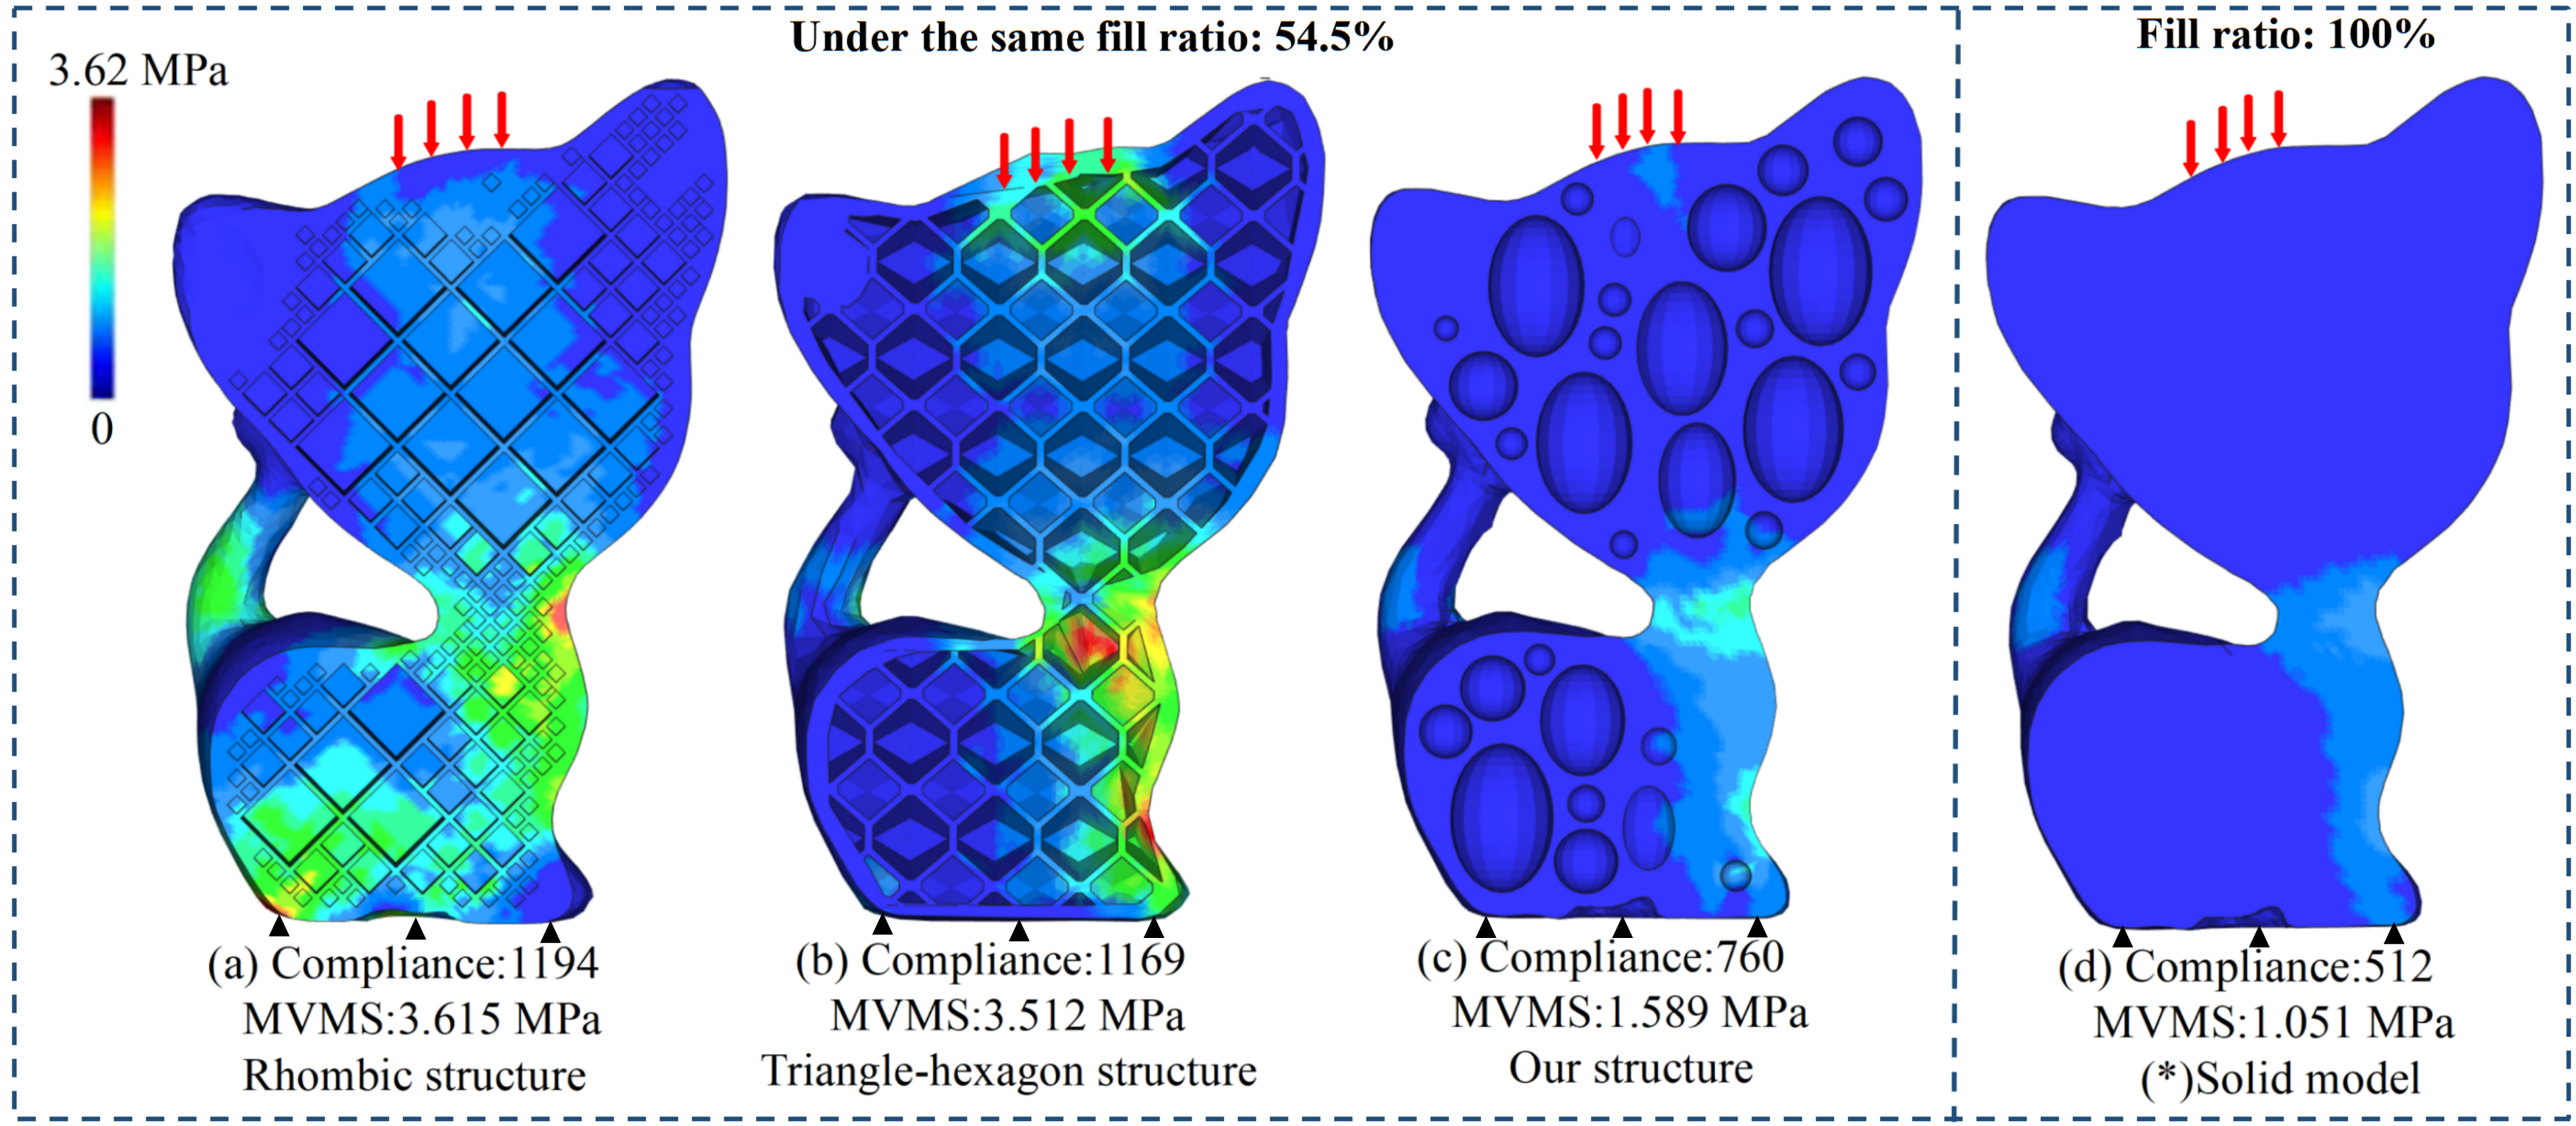
\includegraphics[width=0.8 \textwidth]{./figures/self-support/fig11.png}
    \caption{与相关自支撑空心轻量化方法的比较~\cite{wu2016self,xu2021support}}
    \label{fig:10}
    \end {center}
\end{figure*}

本文方法还与一些非自支撑结构进行了比较,包括蜂窝结构~\cite{10.1145/2601097.2601168}和基于TPMS的结构~\cite{hu2020efficient},如图~\ref{fig:11}所示。
蜂窝结构通过启发式算法进行优化,需要在每次迭代中进行耗时的重网格化。相比之下,所提出的结构可以通过函数进行表示、设计和优化,有利于数值计算的稳定性和快速收敛。
基于TPMS的结构可以使用连续表示自动优化,但由于受TPMS构造的限制,该结构在狭窄和薄弱部位容易出现脆弱性。
比较结果表明,所提出的自支撑结构刚度优于其他结构。主要原因是,该自支撑结构可以直接在函数上进行解析计算,并具有更多可优化的自由度,包括形状(椭球体尺寸)、位置(椭球体位置)和拓扑(椭球体数量)。
在相同45.3\%的填充比下,所提出结构的MVMS和填充比更接近于实心模型(填充比100\%)。
为了更清晰地说明,图~\ref{fig:14}中绘制了这些方法的MVMS直方图。直方图清楚地显示,所提出的结果具有最佳性能,与实心模型相当。
上述相关方法的总结列于表~\ref{T:table2}中。该方法在自支撑性、强度导向性、表示、优化和可优化自由度等方面具有明显优势。

\begin{figure*}[b]
    \begin {center}
    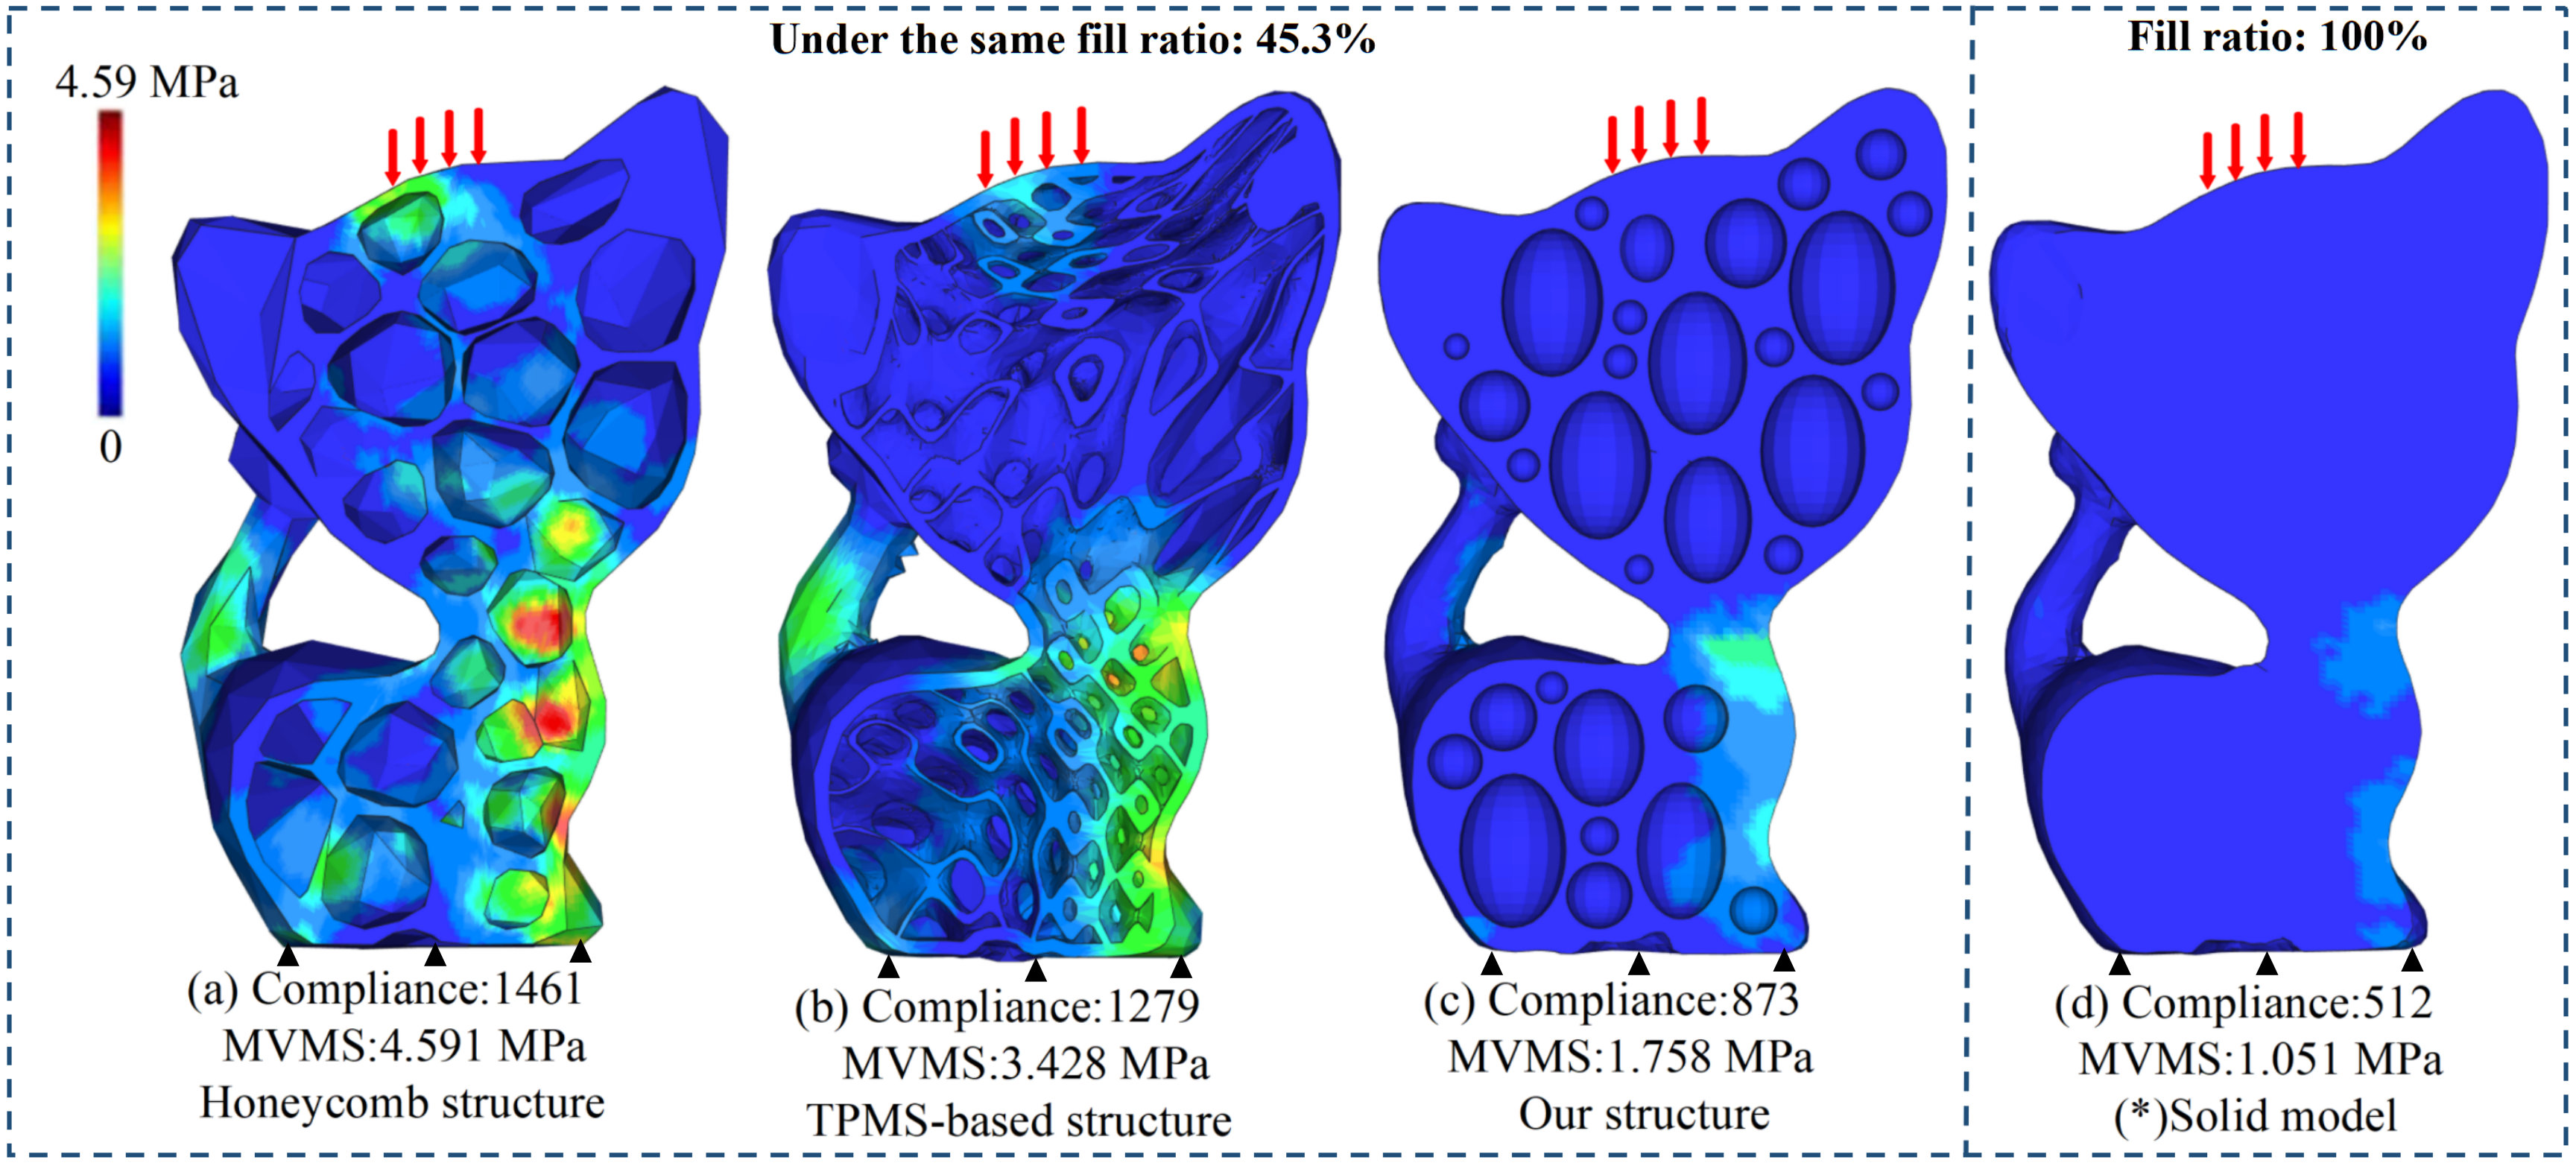
\includegraphics[width=0.8 \textwidth]{./figures/self-support/fig12.png}
    \caption{与相关非自支撑轻量化方法~\cite{10.1145/2601097.2601168,hu2020efficient}的比较}
    \label{fig:11}
    \end {center}
\end{figure*}

\begin{table*}[htbp]
  \centering
  \centering
  \fontsize{7}{8}\selectfont
  \caption{相关方法的定性比较}
  \label{T:table2}
  \renewcommand{\arraystretch}{1.5}
  \setlength{\tabcolsep}{1.8mm}{
  \resizebox{1.0\linewidth}{!}{
      \begin{tabular}{c|c|c|c|c|c}
          \toprule
          \textbf{方法}                                    & \textbf{自支撑性}     & \textbf{强度优化}   & \textbf{表示方法}      & \textbf{优化形式}       & \textbf{优化自由度}         \\ 
          \midrule
          Honeycomb structures in \cite{10.1145/2601097.2601168}      & ×                   & \checkmark          & 离散            & 启发式          & 3D (几何+拓扑)                   \\
          Rhombic structures in \cite{wu2016self}                     & \checkmark          & \checkmark          & 离散            & 自动          & 3D (几何+拓扑)
          \\
          Support-free hollowing structures in \cite{wang2018support} & \checkmark          & ×                   & 离散            & none               & none
          \\
          Elliptical cylinder structures in \cite{lee2018support}     & \checkmark          & ×                   & 离散            & none               & none                                  \\
          TPMS-based structures in \cite{hu2020efficient}             & ×                   & \checkmark          & 连续           & 自动          & 3D (几何+拓扑)                   \\
          Triangle-hexagon structures in \cite{xu2021support}         & \checkmark          & \checkmark          & 离散            & none               & none                                  \\
          \midrule
          \textbf{本文方法}                                        & \textbf{\checkmark} & \textbf{\checkmark} & \textbf{连续} & \textbf{自动} & \textbf{3D (几何+位置+拓扑)} \\ 
          \bottomrule
      \end{tabular}}}
\end{table*}

\begin{figure}[htbp]
  \begin {center}
  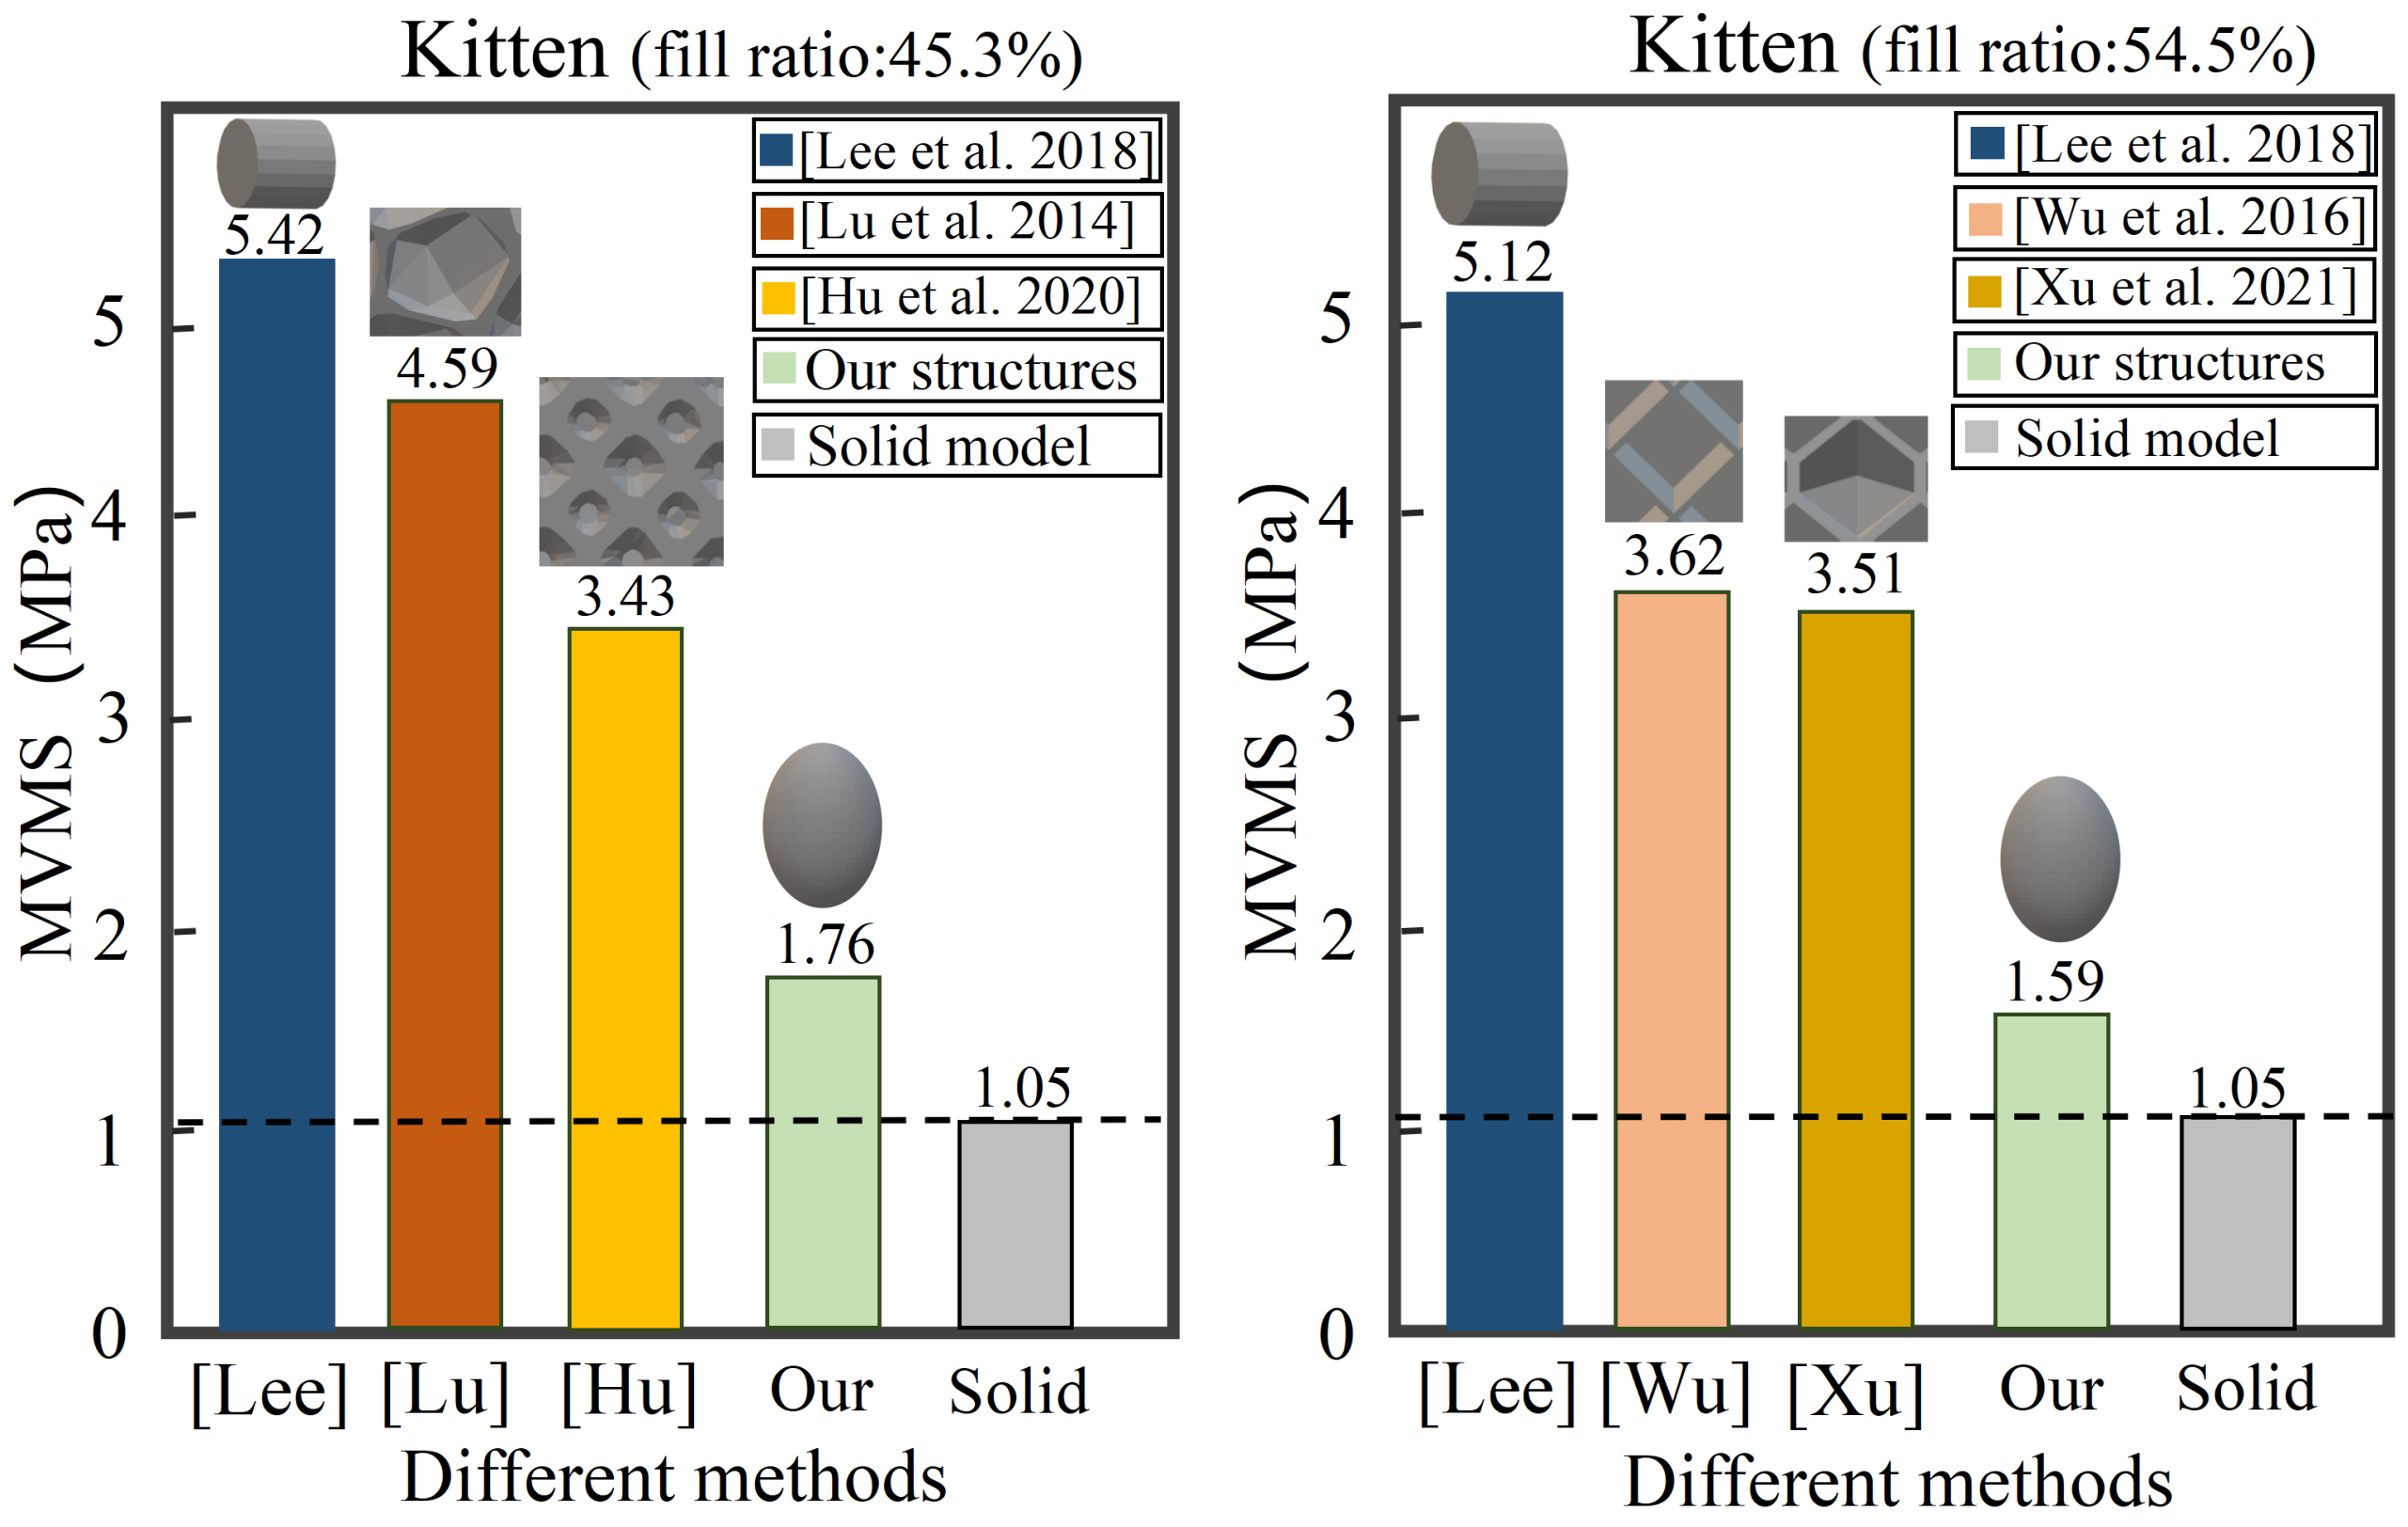
\includegraphics[width=0.8 \textwidth]{./figures/self-support/fig14.png}
  \caption{相同填充比例下不同方法\cite{xu2021support,10.1145/2601097.2601168,wu2016self,hu2020efficient}的MVMS比较直方图}
  % \caption{Histograms of MVMS under the same fill ratio (left:45.3$\%$, right:54.5$\%$). Our structures have the smallest MVMS among the related methods, including
  %     the elliptical cylinder structure \cite{lee2018support},
  %     the Triangle-hexagon structure \cite{xu2021support},
  %     the Honeycomb structure \cite{10.1145/2601097.2601168},
  %     the Rhombic structure \cite{wu2016self} and
  %     the TPMS-based structure \cite{hu2020efficient}.
  %     Our structures are comparable to the solid model.}
  \label{fig:14}
  \end {center}
\end{figure}

\begin{figure}[htbp]
  \begin {center}
  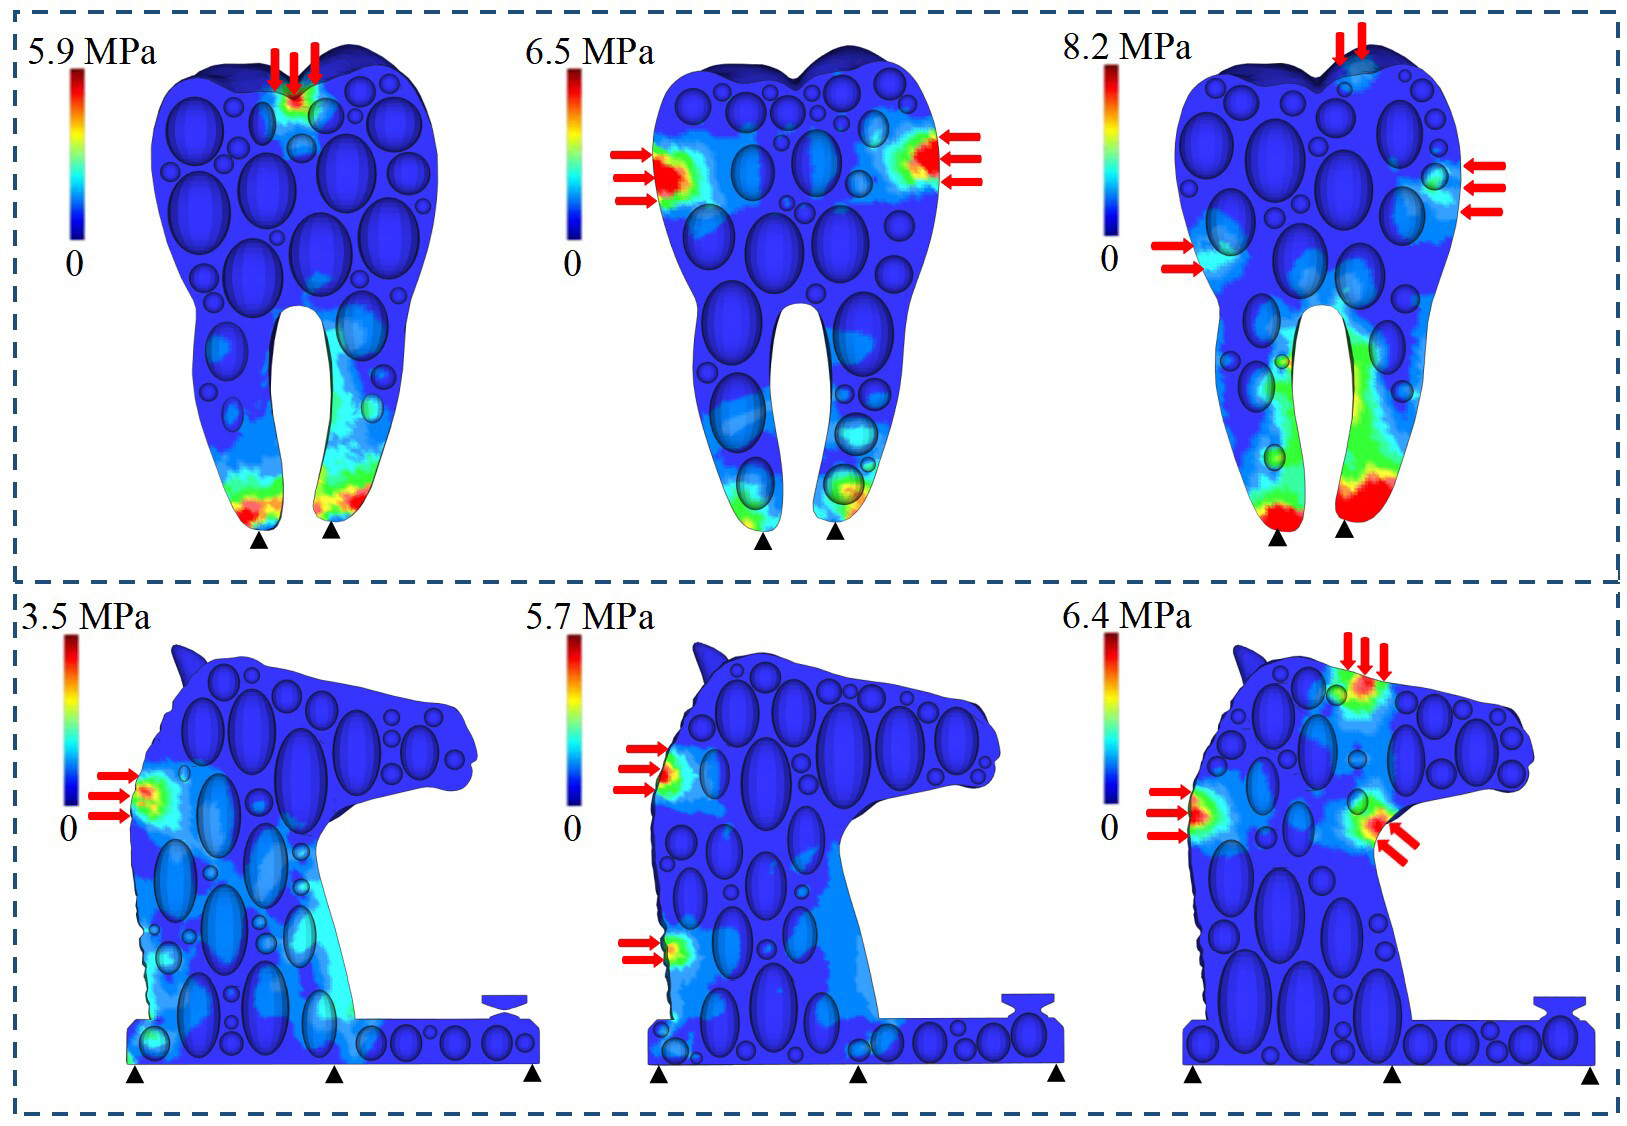
\includegraphics[width=0.9 \textwidth]{./figures/self-support/fig13.png}
  \caption{不同受力方向下的优化结构}
  \label{fig12}
  \end {center}
\end{figure}
所提出的框架支持多种载荷工况。为验证该方法在不同载荷条件下的有效性,如图~\ref{fig12}所示,对其进行了进一步测试。在不同工况下,该方法表现良好,并获得了给定载荷条件下的最优结构。
外力方向没有限制,与椭球体或制造方向无关。
该方法采用的椭球体为各向异性孔隙,当其与应力方向一致时,其机械性能优于等向孔隙。
此外,优化后的模型可通过常见的FDM 3D打印技术制造。
为评估可行性,如图~\ref{fig:15}所示,使用FDM 3D打印机打印了几个优化后的模型。在所有实验中,内部结构均可良好打印,无需额外支撑。
此外,如图~\ref{fig:16}所示,使用RG1-5微型计算机控制电子万能试验机对3D打印模型进行了测试,该结构的机械性能与实心模型相当。两种模型在高荷载下都保持良好状态,即使试验机达到最大5000N的力,主体结构仍然完好。
因此,所提出的方法得到的优化结构是可信和可行的。

\begin{figure*}[htbp]
  \begin {center}
  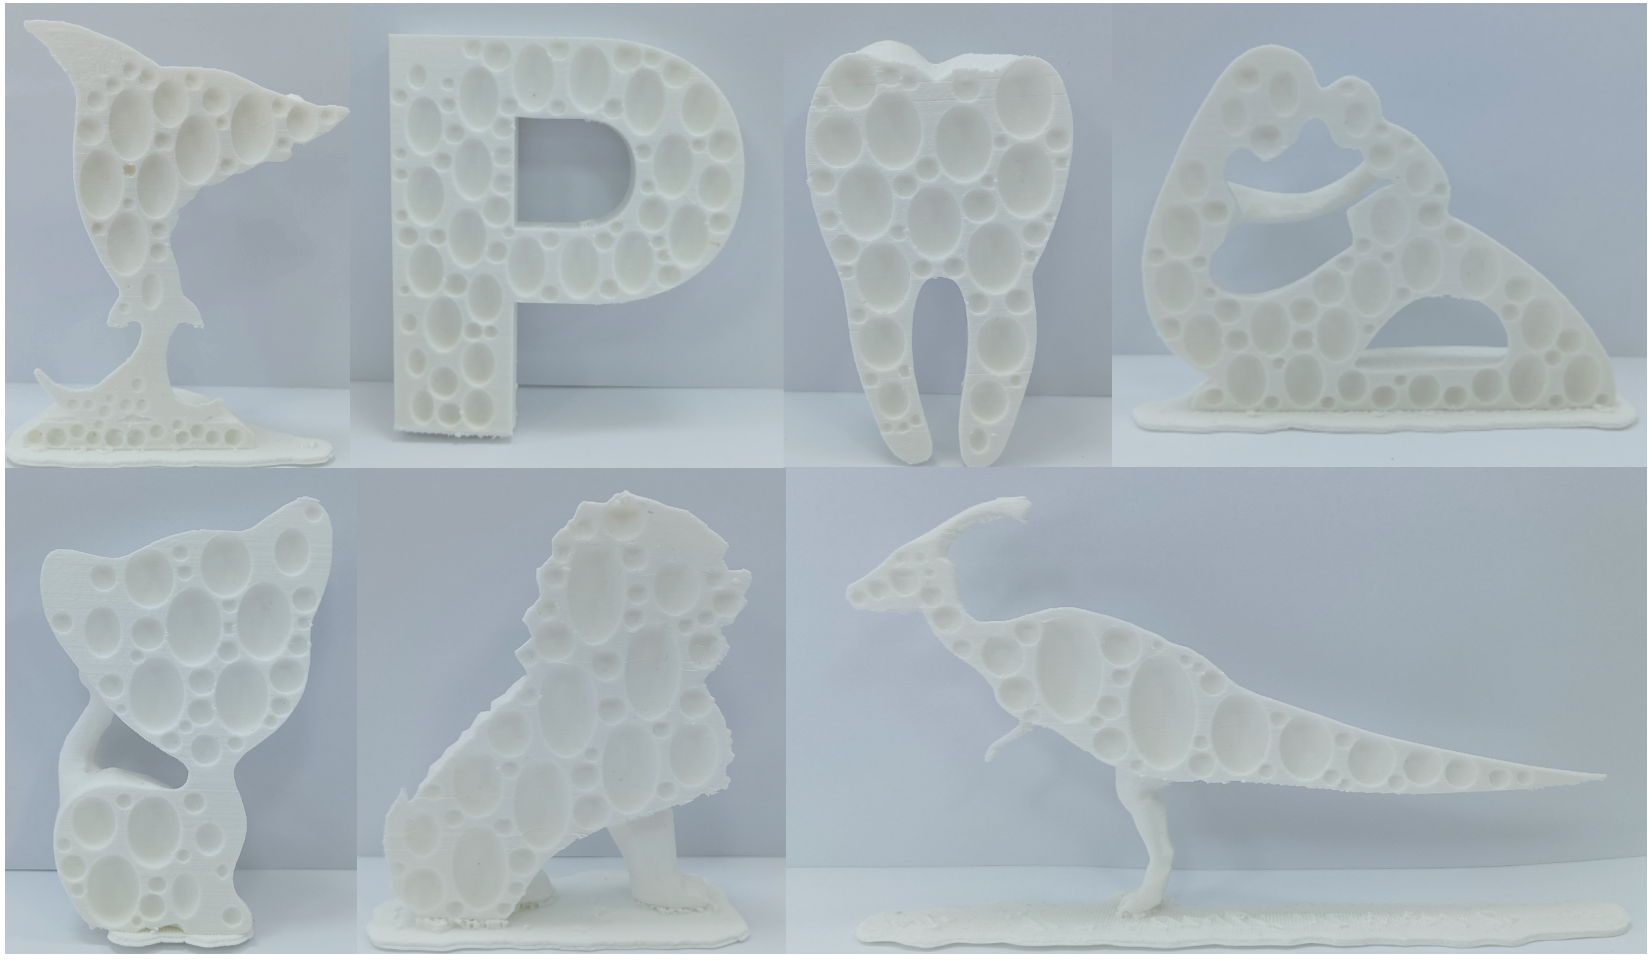
\includegraphics[width=0.9\textwidth]{./figures/self-support/fig16.png}
  \caption{带有椭球形空腔的优化模型的3D打印结果}
  \label{fig:15}
  \end {center}
\end{figure*}

\begin{figure}[htbp]
  \begin {center}
  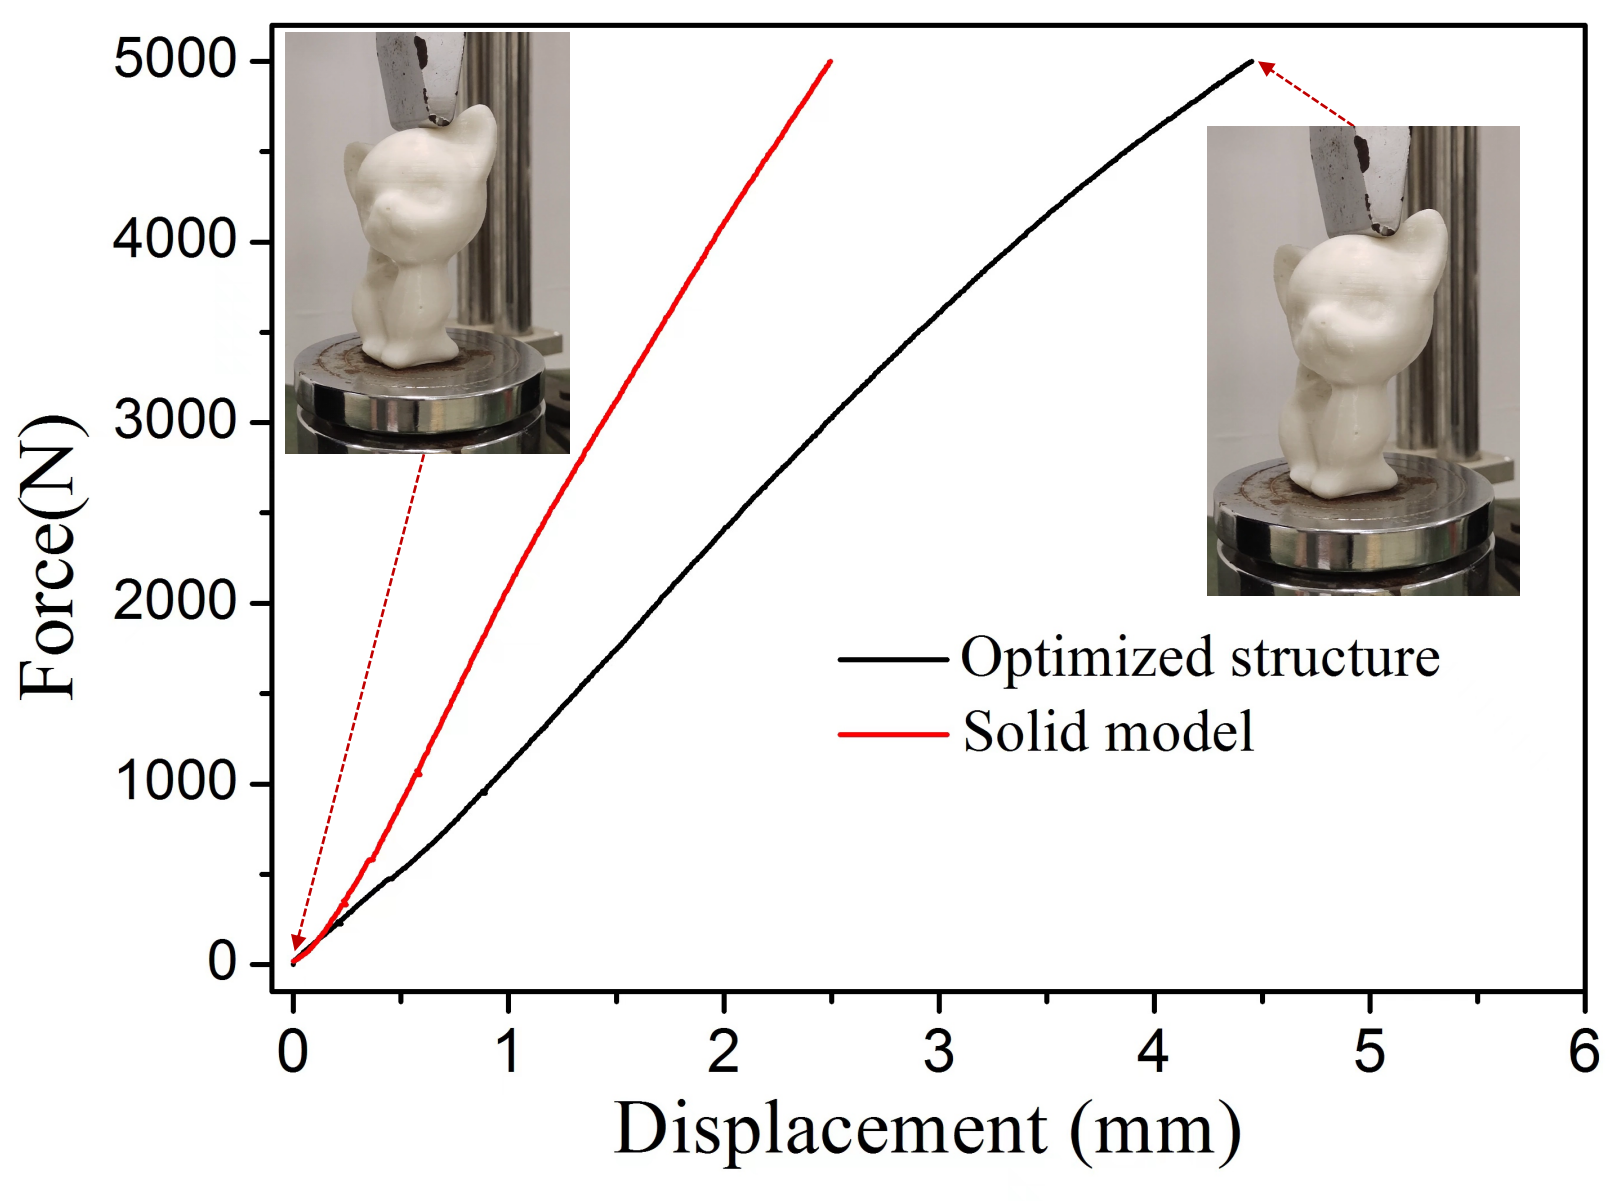
\includegraphics[width=0.6 \textwidth]{./figures/self-support/fig15.png}
  \caption{3D打印模型的实际应力测试 }
  \label{fig:16}
  \end {center}
\end{figure}

\section{本章小结}
本章节提出了一种基于椭球雕刻的无网格自支撑空心化框架。
与现有基于有限元的方法相比,该框架直接在连续函数上进行自支撑空心化的设计和优化,无需耗时的重网格化,大幅提高了空心化问题的有效性和效率。
该框架可自动优化椭球形空腔的形状、位置和拓扑结构,从而得到性能优异的优化自支撑结构。
一系列实验结果证明了该框架的有效性。